% Options for packages loaded elsewhere
% Options for packages loaded elsewhere
\PassOptionsToPackage{unicode}{hyperref}
\PassOptionsToPackage{hyphens}{url}
\PassOptionsToPackage{dvipsnames,svgnames,x11names}{xcolor}
%
\documentclass[
  letterpaper,
  DIV=11,
  numbers=noendperiod]{scrartcl}
\usepackage{xcolor}
\usepackage{amsmath,amssymb}
\setcounter{secnumdepth}{5}
\usepackage{iftex}
\ifPDFTeX
  \usepackage[T1]{fontenc}
  \usepackage[utf8]{inputenc}
  \usepackage{textcomp} % provide euro and other symbols
\else % if luatex or xetex
  \usepackage{unicode-math} % this also loads fontspec
  \defaultfontfeatures{Scale=MatchLowercase}
  \defaultfontfeatures[\rmfamily]{Ligatures=TeX,Scale=1}
\fi
\usepackage{lmodern}
\ifPDFTeX\else
  % xetex/luatex font selection
\fi
% Use upquote if available, for straight quotes in verbatim environments
\IfFileExists{upquote.sty}{\usepackage{upquote}}{}
\IfFileExists{microtype.sty}{% use microtype if available
  \usepackage[]{microtype}
  \UseMicrotypeSet[protrusion]{basicmath} % disable protrusion for tt fonts
}{}
\makeatletter
\@ifundefined{KOMAClassName}{% if non-KOMA class
  \IfFileExists{parskip.sty}{%
    \usepackage{parskip}
  }{% else
    \setlength{\parindent}{0pt}
    \setlength{\parskip}{6pt plus 2pt minus 1pt}}
}{% if KOMA class
  \KOMAoptions{parskip=half}}
\makeatother
% Make \paragraph and \subparagraph free-standing
\makeatletter
\ifx\paragraph\undefined\else
  \let\oldparagraph\paragraph
  \renewcommand{\paragraph}{
    \@ifstar
      \xxxParagraphStar
      \xxxParagraphNoStar
  }
  \newcommand{\xxxParagraphStar}[1]{\oldparagraph*{#1}\mbox{}}
  \newcommand{\xxxParagraphNoStar}[1]{\oldparagraph{#1}\mbox{}}
\fi
\ifx\subparagraph\undefined\else
  \let\oldsubparagraph\subparagraph
  \renewcommand{\subparagraph}{
    \@ifstar
      \xxxSubParagraphStar
      \xxxSubParagraphNoStar
  }
  \newcommand{\xxxSubParagraphStar}[1]{\oldsubparagraph*{#1}\mbox{}}
  \newcommand{\xxxSubParagraphNoStar}[1]{\oldsubparagraph{#1}\mbox{}}
\fi
\makeatother

\usepackage{color}
\usepackage{fancyvrb}
\newcommand{\VerbBar}{|}
\newcommand{\VERB}{\Verb[commandchars=\\\{\}]}
\DefineVerbatimEnvironment{Highlighting}{Verbatim}{commandchars=\\\{\}}
% Add ',fontsize=\small' for more characters per line
\usepackage{framed}
\definecolor{shadecolor}{RGB}{241,243,245}
\newenvironment{Shaded}{\begin{snugshade}}{\end{snugshade}}
\newcommand{\AlertTok}[1]{\textcolor[rgb]{0.68,0.00,0.00}{#1}}
\newcommand{\AnnotationTok}[1]{\textcolor[rgb]{0.37,0.37,0.37}{#1}}
\newcommand{\AttributeTok}[1]{\textcolor[rgb]{0.40,0.45,0.13}{#1}}
\newcommand{\BaseNTok}[1]{\textcolor[rgb]{0.68,0.00,0.00}{#1}}
\newcommand{\BuiltInTok}[1]{\textcolor[rgb]{0.00,0.23,0.31}{#1}}
\newcommand{\CharTok}[1]{\textcolor[rgb]{0.13,0.47,0.30}{#1}}
\newcommand{\CommentTok}[1]{\textcolor[rgb]{0.37,0.37,0.37}{#1}}
\newcommand{\CommentVarTok}[1]{\textcolor[rgb]{0.37,0.37,0.37}{\textit{#1}}}
\newcommand{\ConstantTok}[1]{\textcolor[rgb]{0.56,0.35,0.01}{#1}}
\newcommand{\ControlFlowTok}[1]{\textcolor[rgb]{0.00,0.23,0.31}{\textbf{#1}}}
\newcommand{\DataTypeTok}[1]{\textcolor[rgb]{0.68,0.00,0.00}{#1}}
\newcommand{\DecValTok}[1]{\textcolor[rgb]{0.68,0.00,0.00}{#1}}
\newcommand{\DocumentationTok}[1]{\textcolor[rgb]{0.37,0.37,0.37}{\textit{#1}}}
\newcommand{\ErrorTok}[1]{\textcolor[rgb]{0.68,0.00,0.00}{#1}}
\newcommand{\ExtensionTok}[1]{\textcolor[rgb]{0.00,0.23,0.31}{#1}}
\newcommand{\FloatTok}[1]{\textcolor[rgb]{0.68,0.00,0.00}{#1}}
\newcommand{\FunctionTok}[1]{\textcolor[rgb]{0.28,0.35,0.67}{#1}}
\newcommand{\ImportTok}[1]{\textcolor[rgb]{0.00,0.46,0.62}{#1}}
\newcommand{\InformationTok}[1]{\textcolor[rgb]{0.37,0.37,0.37}{#1}}
\newcommand{\KeywordTok}[1]{\textcolor[rgb]{0.00,0.23,0.31}{\textbf{#1}}}
\newcommand{\NormalTok}[1]{\textcolor[rgb]{0.00,0.23,0.31}{#1}}
\newcommand{\OperatorTok}[1]{\textcolor[rgb]{0.37,0.37,0.37}{#1}}
\newcommand{\OtherTok}[1]{\textcolor[rgb]{0.00,0.23,0.31}{#1}}
\newcommand{\PreprocessorTok}[1]{\textcolor[rgb]{0.68,0.00,0.00}{#1}}
\newcommand{\RegionMarkerTok}[1]{\textcolor[rgb]{0.00,0.23,0.31}{#1}}
\newcommand{\SpecialCharTok}[1]{\textcolor[rgb]{0.37,0.37,0.37}{#1}}
\newcommand{\SpecialStringTok}[1]{\textcolor[rgb]{0.13,0.47,0.30}{#1}}
\newcommand{\StringTok}[1]{\textcolor[rgb]{0.13,0.47,0.30}{#1}}
\newcommand{\VariableTok}[1]{\textcolor[rgb]{0.07,0.07,0.07}{#1}}
\newcommand{\VerbatimStringTok}[1]{\textcolor[rgb]{0.13,0.47,0.30}{#1}}
\newcommand{\WarningTok}[1]{\textcolor[rgb]{0.37,0.37,0.37}{\textit{#1}}}

\usepackage{longtable,booktabs,array}
\usepackage{calc} % for calculating minipage widths
% Correct order of tables after \paragraph or \subparagraph
\usepackage{etoolbox}
\makeatletter
\patchcmd\longtable{\par}{\if@noskipsec\mbox{}\fi\par}{}{}
\makeatother
% Allow footnotes in longtable head/foot
\IfFileExists{footnotehyper.sty}{\usepackage{footnotehyper}}{\usepackage{footnote}}
\makesavenoteenv{longtable}
\usepackage{graphicx}
\makeatletter
\newsavebox\pandoc@box
\newcommand*\pandocbounded[1]{% scales image to fit in text height/width
  \sbox\pandoc@box{#1}%
  \Gscale@div\@tempa{\textheight}{\dimexpr\ht\pandoc@box+\dp\pandoc@box\relax}%
  \Gscale@div\@tempb{\linewidth}{\wd\pandoc@box}%
  \ifdim\@tempb\p@<\@tempa\p@\let\@tempa\@tempb\fi% select the smaller of both
  \ifdim\@tempa\p@<\p@\scalebox{\@tempa}{\usebox\pandoc@box}%
  \else\usebox{\pandoc@box}%
  \fi%
}
% Set default figure placement to htbp
\def\fps@figure{htbp}
\makeatother





\setlength{\emergencystretch}{3em} % prevent overfull lines

\providecommand{\tightlist}{%
  \setlength{\itemsep}{0pt}\setlength{\parskip}{0pt}}



 


\usepackage{booktabs}
\usepackage{longtable}
\usepackage{array}
\usepackage{multirow}
\usepackage{wrapfig}
\usepackage{float}
\usepackage{colortbl}
\usepackage{pdflscape}
\usepackage{tabu}
\usepackage{threeparttable}
\usepackage{threeparttablex}
\usepackage[normalem]{ulem}
\usepackage{makecell}
\usepackage{xcolor}
\KOMAoption{captions}{tableheading}
\makeatletter
\@ifpackageloaded{caption}{}{\usepackage{caption}}
\AtBeginDocument{%
\ifdefined\contentsname
  \renewcommand*\contentsname{Table of contents}
\else
  \newcommand\contentsname{Table of contents}
\fi
\ifdefined\listfigurename
  \renewcommand*\listfigurename{List of Figures}
\else
  \newcommand\listfigurename{List of Figures}
\fi
\ifdefined\listtablename
  \renewcommand*\listtablename{List of Tables}
\else
  \newcommand\listtablename{List of Tables}
\fi
\ifdefined\figurename
  \renewcommand*\figurename{Figure}
\else
  \newcommand\figurename{Figure}
\fi
\ifdefined\tablename
  \renewcommand*\tablename{Table}
\else
  \newcommand\tablename{Table}
\fi
}
\@ifpackageloaded{float}{}{\usepackage{float}}
\floatstyle{ruled}
\@ifundefined{c@chapter}{\newfloat{codelisting}{h}{lop}}{\newfloat{codelisting}{h}{lop}[chapter]}
\floatname{codelisting}{Listing}
\newcommand*\listoflistings{\listof{codelisting}{List of Listings}}
\makeatother
\makeatletter
\makeatother
\makeatletter
\@ifpackageloaded{caption}{}{\usepackage{caption}}
\@ifpackageloaded{subcaption}{}{\usepackage{subcaption}}
\makeatother
\usepackage{bookmark}
\IfFileExists{xurl.sty}{\usepackage{xurl}}{} % add URL line breaks if available
\urlstyle{same}
\hypersetup{
  pdftitle={GRA4158 Marketing - Analysis of Experiments, Portfolio 3},
  pdfauthor={Vilijam Cekov, Luiz Felipe De Souza Simao},
  colorlinks=true,
  linkcolor={blue},
  filecolor={Maroon},
  citecolor={Blue},
  urlcolor={Blue},
  pdfcreator={LaTeX via pandoc}}


\title{GRA4158 Marketing - Analysis of Experiments, Portfolio 3}
\author{Vilijam Cekov, Luiz Felipe De Souza Simao}
\date{}
\begin{document}
\maketitle

\renewcommand*\contentsname{Table of contents}
{
\hypersetup{linkcolor=}
\setcounter{tocdepth}{3}
\tableofcontents
}

\section{Import Data}\label{import-data}

\begin{Shaded}
\begin{Highlighting}[]
\NormalTok{casedata\_task3 }\OtherTok{\textless{}{-}} \FunctionTok{read.csv}\NormalTok{(}\StringTok{"CaseData\_Task3.csv"}\NormalTok{, }\AttributeTok{stringsAsFactors =} \ConstantTok{FALSE}\NormalTok{)}

\CommentTok{\# Display the structure of the data to verify column names}
\FunctionTok{str}\NormalTok{(casedata\_task3)}
\end{Highlighting}
\end{Shaded}

\begin{verbatim}
'data.frame':   5000 obs. of  22 variables:
 $ X1 : num  23.8 21 22.8 25.8 22.9 24.9 24.1 21.4 24.8 23.8 ...
 $ X2 : num  13.7 14.4 11.5 13.5 13.6 12.9 11.8 12.4 14.2 15.9 ...
 $ X3 : num  22.5 21.5 20.6 22.7 21.6 19.4 22.9 19.5 21.6 23.4 ...
 $ X4 : num  16.2 14.5 14.7 15.8 17.5 13.8 17 13.8 15.5 16.8 ...
 $ X5 : int  0 0 0 1 1 0 1 0 0 1 ...
 $ X6 : num  22.9 23.4 20.2 22.5 23.5 21.1 24.6 20 23.9 20 ...
 $ X7 : num  11.6 11.2 9.6 11.5 12.7 9.6 12.9 9.5 11.4 9.2 ...
 $ X8 : num  10.1 12.8 9.7 10.3 12.3 6.3 9.6 7.4 10.6 11.9 ...
 $ X9 : num  18.9 20.2 19 21.9 19.7 15 20.2 17.1 23.8 20.2 ...
 $ X10: num  14.6 13 15.1 18.1 13.7 11.4 15.2 10.3 19.7 14.2 ...
 $ X11: num  13.1 13.7 14.6 14.2 14.5 12 14.1 11.4 16.4 13.6 ...
 $ X12: num  6.2 5.5 6.6 5.3 6.7 3.8 5.9 5 8.8 6.5 ...
 $ X13: num  14 13.5 16.6 13.3 14.8 11.8 13.8 12.9 15.2 15.3 ...
 $ X14: num  5.4 3.7 7.3 4.1 4.2 4.4 4.5 3.7 5.1 5.4 ...
 $ X15: num  11.6 9 13.4 10.2 10.5 10.6 11.8 9.6 11.8 11.7 ...
 $ X16: num  10.9 9.9 12.4 10.6 10.2 9.2 11.2 8.9 11 11.7 ...
 $ X17: num  12 12.4 13.3 11.1 11.8 10.7 12.6 12 11.7 12.9 ...
 $ X18: num  8.6 7.4 8.1 5.9 8.5 6.8 7.5 7.1 6.6 8.1 ...
 $ X19: num  12.3 12.1 11.8 10.3 12.8 10.2 11.1 10.8 11 12 ...
 $ X20: int  0 0 1 1 0 1 0 0 1 0 ...
 $ y  : int  1463 2410 659 2202 2196 2329 1993 2467 1644 1499 ...
 $ d  : int  0 1 1 1 0 1 1 1 0 1 ...
\end{verbatim}

\begin{Shaded}
\begin{Highlighting}[]
\CommentTok{\# Check the first few rows}
\FunctionTok{head}\NormalTok{(casedata\_task3)}
\end{Highlighting}
\end{Shaded}

\begin{verbatim}
    X1   X2   X3   X4 X5   X6   X7   X8   X9  X10  X11 X12  X13 X14  X15  X16
1 23.8 13.7 22.5 16.2  0 22.9 11.6 10.1 18.9 14.6 13.1 6.2 14.0 5.4 11.6 10.9
2 21.0 14.4 21.5 14.5  0 23.4 11.2 12.8 20.2 13.0 13.7 5.5 13.5 3.7  9.0  9.9
3 22.8 11.5 20.6 14.7  0 20.2  9.6  9.7 19.0 15.1 14.6 6.6 16.6 7.3 13.4 12.4
4 25.8 13.5 22.7 15.8  1 22.5 11.5 10.3 21.9 18.1 14.2 5.3 13.3 4.1 10.2 10.6
5 22.9 13.6 21.6 17.5  1 23.5 12.7 12.3 19.7 13.7 14.5 6.7 14.8 4.2 10.5 10.2
6 24.9 12.9 19.4 13.8  0 21.1  9.6  6.3 15.0 11.4 12.0 3.8 11.8 4.4 10.6  9.2
   X17 X18  X19 X20    y d
1 12.0 8.6 12.3   0 1463 0
2 12.4 7.4 12.1   0 2410 1
3 13.3 8.1 11.8   1  659 1
4 11.1 5.9 10.3   1 2202 1
5 11.8 8.5 12.8   0 2196 0
6 10.7 6.8 10.2   1 2329 1
\end{verbatim}

\section{Estimate the treatment effect using simple linear Regression
Adjustment}\label{estimate-the-treatment-effect-using-simple-linear-regression-adjustment}

The estimate for the discount coefficient is the Regression Adjustment
ATE

\begin{Shaded}
\begin{Highlighting}[]
\NormalTok{model\_adj }\OtherTok{\textless{}{-}} \FunctionTok{lm}\NormalTok{(y }\SpecialCharTok{\textasciitilde{}}\NormalTok{ d }\SpecialCharTok{+}\NormalTok{ X1 }\SpecialCharTok{+}\NormalTok{ X2 }\SpecialCharTok{+}\NormalTok{ X3 }\SpecialCharTok{+}\NormalTok{ X4 }\SpecialCharTok{+}\NormalTok{ X5 }\SpecialCharTok{+}\NormalTok{ X6 }\SpecialCharTok{+}\NormalTok{ X7 }\SpecialCharTok{+}\NormalTok{ X8 }\SpecialCharTok{+}\NormalTok{ X9 }\SpecialCharTok{+}\NormalTok{ X10 }\SpecialCharTok{+}
\NormalTok{                 X11 }\SpecialCharTok{+}\NormalTok{ X12 }\SpecialCharTok{+}\NormalTok{ X13 }\SpecialCharTok{+}\NormalTok{ X14 }\SpecialCharTok{+}\NormalTok{ X15 }\SpecialCharTok{+}\NormalTok{ X16 }\SpecialCharTok{+}\NormalTok{ X17 }\SpecialCharTok{+}\NormalTok{ X18 }\SpecialCharTok{+}\NormalTok{ X19 }\SpecialCharTok{+}\NormalTok{ X20,}
                 \AttributeTok{data =}\NormalTok{ casedata\_task3)}

\FunctionTok{coeftest}\NormalTok{(model\_adj)[}\StringTok{"d"}\NormalTok{, , drop }\OtherTok{=} \ConstantTok{FALSE}\NormalTok{]}
\end{Highlighting}
\end{Shaded}

\begin{verbatim}
  Estimate Std. Error  t value    Pr(>|t|)
d 15.15365   5.704223 2.656566 0.007919282
\end{verbatim}

Extract the ATE value from the regression and calculate robust standard
errors using the HC3 estimator, which is more reliable in small samples
and with heteroskedasticity.

\begin{Shaded}
\begin{Highlighting}[]
\FunctionTok{coeftest}\NormalTok{(model\_adj, }\AttributeTok{vcov =} \FunctionTok{vcovHC}\NormalTok{(model\_adj, }\AttributeTok{type =} \StringTok{"HC3"}\NormalTok{))}
\end{Highlighting}
\end{Shaded}

\begin{verbatim}

t test of coefficients:

              Estimate Std. Error  t value  Pr(>|t|)    
(Intercept) 4697.04561   76.15859  61.6745 < 2.2e-16 ***
d             15.15365    5.80286   2.6114  0.009044 ** 
X1             3.06184    1.51318   2.0235  0.043080 *  
X2            -1.56049    1.81397  -0.8603  0.389687    
X3             1.36316    1.83034   0.7448  0.456453    
X4            -2.84763    1.74765  -1.6294  0.103291    
X5            36.24104    5.67533   6.3857 1.861e-10 ***
X6            -1.72139    1.71427  -1.0042  0.315354    
X7            21.87065    1.79930  12.1551 < 2.2e-16 ***
X8            -1.31713    1.85035  -0.7118  0.476607    
X9             0.87561    1.80426   0.4853  0.627484    
X10           -1.33908    1.86892  -0.7165  0.473716    
X11           -0.10716    3.77342  -0.0284  0.977345    
X12            1.27229    4.16008   0.3058  0.759745    
X13           -7.17543    3.72007  -1.9288  0.053807 .  
X14         -304.00261    3.64002 -83.5167 < 2.2e-16 ***
X15         -133.66096    3.78412 -35.3216 < 2.2e-16 ***
X16            0.51387    3.54850   0.1448  0.884863    
X17            1.52685    3.65959   0.4172  0.676537    
X18           -1.88837    3.63423  -0.5196  0.603362    
X19            0.87427    3.36898   0.2595  0.795255    
X20          -26.96513    5.41454  -4.9801 6.569e-07 ***
---
Signif. codes:  0 '***' 0.001 '**' 0.01 '*' 0.05 '.' 0.1 ' ' 1
\end{verbatim}

\begin{verbatim}
The estimated Average Treatment Effect (ATE) for the treatment is: $15.15
\end{verbatim}

\section{Propensity Score Estimation and Overlap
Diagnostic}\label{propensity-score-estimation-and-overlap-diagnostic}

Before implementing matching or weighting, I first estimate the
propensity scores and evaluate the common support assumption. This step
is a necessary prerequisite to ensure that there is sufficient overlap
in the covariate distributions between the treated and control groups

\begin{Shaded}
\begin{Highlighting}[]
\CommentTok{\# Complete{-}case sample for IPW variables}
\NormalTok{ipw\_vars }\OtherTok{\textless{}{-}} \FunctionTok{c}\NormalTok{(}\StringTok{"y"}\NormalTok{, }\StringTok{"d"}\NormalTok{, }\FunctionTok{paste0}\NormalTok{(}\StringTok{"X"}\NormalTok{, }\DecValTok{1}\SpecialCharTok{:}\DecValTok{20}\NormalTok{))}
\NormalTok{df\_ipw }\OtherTok{\textless{}{-}}\NormalTok{ casedata\_task3[}\FunctionTok{complete.cases}\NormalTok{(casedata\_task3[, ipw\_vars]), ]}

\CommentTok{\# 1) Estimate propensity scores with logistic regression}
\NormalTok{ps\_model }\OtherTok{\textless{}{-}} \FunctionTok{glm}\NormalTok{(}
\NormalTok{  d }\SpecialCharTok{\textasciitilde{}}\NormalTok{ X1 }\SpecialCharTok{+}\NormalTok{ X2 }\SpecialCharTok{+}\NormalTok{ X3 }\SpecialCharTok{+}\NormalTok{ X4 }\SpecialCharTok{+}\NormalTok{ X5 }\SpecialCharTok{+}\NormalTok{ X6 }\SpecialCharTok{+}\NormalTok{ X7 }\SpecialCharTok{+}\NormalTok{ X8 }\SpecialCharTok{+}\NormalTok{ X9 }\SpecialCharTok{+}\NormalTok{ X10 }\SpecialCharTok{+}
\NormalTok{      X11 }\SpecialCharTok{+}\NormalTok{ X12 }\SpecialCharTok{+}\NormalTok{ X13 }\SpecialCharTok{+}\NormalTok{ X14 }\SpecialCharTok{+}\NormalTok{ X15 }\SpecialCharTok{+}\NormalTok{ X16 }\SpecialCharTok{+}\NormalTok{ X17 }\SpecialCharTok{+}\NormalTok{ X18 }\SpecialCharTok{+}\NormalTok{ X19 }\SpecialCharTok{+}\NormalTok{ X20,}
  \AttributeTok{data =}\NormalTok{ df\_ipw,}
  \AttributeTok{family =} \FunctionTok{binomial}\NormalTok{(}\AttributeTok{link =} \StringTok{"logit"}\NormalTok{)}
\NormalTok{)}

\NormalTok{df\_ipw}\SpecialCharTok{$}\NormalTok{ps }\OtherTok{\textless{}{-}} \FunctionTok{predict}\NormalTok{(ps\_model, }\AttributeTok{type =} \StringTok{"response"}\NormalTok{)}

\CommentTok{\# Overlap/common support diagnostic BEFORE trimming}
\FunctionTok{ggplot}\NormalTok{(df\_ipw, }\FunctionTok{aes}\NormalTok{(}\AttributeTok{x =}\NormalTok{ ps, }\AttributeTok{color =} \FunctionTok{factor}\NormalTok{(d), }\AttributeTok{fill =} \FunctionTok{factor}\NormalTok{(d))) }\SpecialCharTok{+}
  \FunctionTok{geom\_density}\NormalTok{(}\AttributeTok{alpha =} \FloatTok{0.25}\NormalTok{) }\SpecialCharTok{+}
  \FunctionTok{labs}\NormalTok{(}
    \AttributeTok{title =} \StringTok{"Propensity Score Overlap (Before Trimming)"}\NormalTok{,}
    \AttributeTok{x =} \StringTok{"Estimated propensity score"}\NormalTok{,}
    \AttributeTok{y =} \StringTok{"Density"}\NormalTok{,}
    \AttributeTok{color =} \StringTok{"Treatment (d)"}\NormalTok{,}
    \AttributeTok{fill =} \StringTok{"Treatment (d)"}
\NormalTok{  ) }\SpecialCharTok{+}
  \FunctionTok{theme\_minimal}\NormalTok{()}
\end{Highlighting}
\end{Shaded}

\pandocbounded{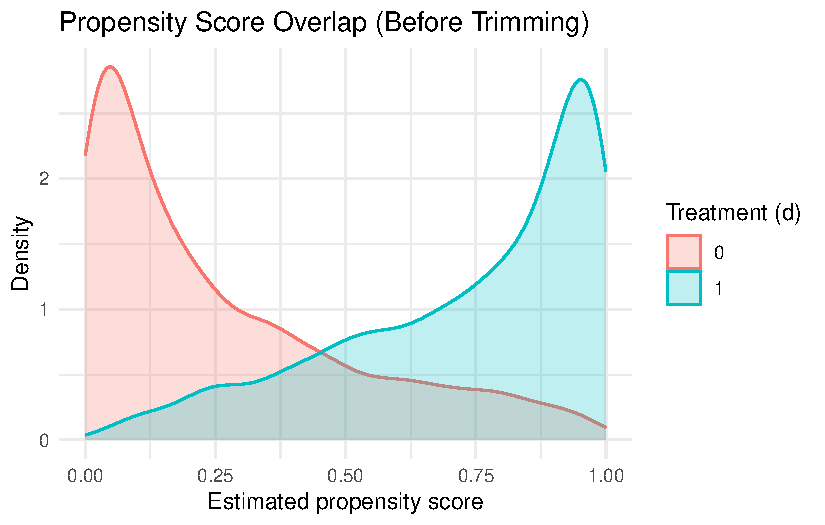
\includegraphics[keepaspectratio]{Portfolio_Task_3-vilijam_files/figure-pdf/unnamed-chunk-5-1.pdf}}

\textbf{Discussion of Overlap Diagnostic}: The density plot of the
estimated propensity scores shows that the treated group (d=1) has a
distribution of scores that is quite different from the control group
(d=0). The treated units tend to have higher propensity scores, while
many control units have scores close to zero. This indicates poor
overlap between the groups, which can lead to issues with both matching
and weighting methods. In particular, IPW may produce extreme weights
for control units with very low propensity scores, leading to unstable
estimates. Matching may also struggle to find good matches for treated
units if the control group is not well represented across the range of
propensity scores. This is a red flag that we may need to consider
trimming the sample or using more robust methods that are less sensitive
to poor overlap, such as AIPW or DML. As such, it is important to
consider that the limited overlap is why both matching and IPW weights
may struggle with this dataset, and why we should be cautious in
interpreting results from those methods.

\section{Matching comparisons}\label{matching-comparisons}

Preparing the data for matching excersises

\begin{Shaded}
\begin{Highlighting}[]
\NormalTok{ps\_formula }\OtherTok{\textless{}{-}}\NormalTok{ d }\SpecialCharTok{\textasciitilde{}}\NormalTok{ X1 }\SpecialCharTok{+}\NormalTok{ X2 }\SpecialCharTok{+}\NormalTok{ X3 }\SpecialCharTok{+}\NormalTok{ X4 }\SpecialCharTok{+}\NormalTok{ X5 }\SpecialCharTok{+}\NormalTok{ X6 }\SpecialCharTok{+}\NormalTok{ X7 }\SpecialCharTok{+}\NormalTok{ X8 }\SpecialCharTok{+}\NormalTok{ X9 }\SpecialCharTok{+}\NormalTok{ X10 }\SpecialCharTok{+}\NormalTok{ X11 }\SpecialCharTok{+} 
\NormalTok{X12 }\SpecialCharTok{+}\NormalTok{ X13 }\SpecialCharTok{+}\NormalTok{ X14 }\SpecialCharTok{+}\NormalTok{ X15 }\SpecialCharTok{+}\NormalTok{ X16 }\SpecialCharTok{+}\NormalTok{ X17 }\SpecialCharTok{+}\NormalTok{ X18 }\SpecialCharTok{+}\NormalTok{ X19 }\SpecialCharTok{+}\NormalTok{ X20}
\end{Highlighting}
\end{Shaded}

\subsection{1:1 Nearest Neighbor Matching WITHOUT
Replacement}\label{nearest-neighbor-matching-without-replacement}

\begin{Shaded}
\begin{Highlighting}[]
\NormalTok{match\_no\_replace }\OtherTok{\textless{}{-}} \FunctionTok{matchit}\NormalTok{(ps\_formula, }
                            \AttributeTok{data =}\NormalTok{ casedata\_task3, }
                            \AttributeTok{method =} \StringTok{"nearest"}\NormalTok{, }
                            \AttributeTok{distance =} \StringTok{"glm"}\NormalTok{,   }\CommentTok{\# Use logistic reg for scores}
                            \AttributeTok{replace =} \ConstantTok{FALSE}\NormalTok{,    }\CommentTok{\# Without replacement}
                            \AttributeTok{ratio =} \DecValTok{1}\NormalTok{)          }\CommentTok{\# 1:1 matching}

\CommentTok{\# View a summary to check covariate balance (ideally Std. Mean Diff \textless{} 0.1)}
\FunctionTok{print}\NormalTok{(}\FunctionTok{summary}\NormalTok{(match\_no\_replace, }\AttributeTok{un =} \ConstantTok{FALSE}\NormalTok{))}
\end{Highlighting}
\end{Shaded}

\begin{verbatim}

Call:
matchit(formula = ps_formula, data = casedata_task3, method = "nearest", 
    distance = "glm", replace = FALSE, ratio = 1)

Summary of Balance for Matched Data:
         Means Treated Means Control Std. Mean Diff. Var. Ratio eCDF Mean
distance        0.7342        0.2657          1.9201     0.9190    0.3878
X1             24.0591       24.0637         -0.0023     0.9305    0.0067
X2             14.1096       14.0910          0.0093     0.9578    0.0048
X3             22.0102       22.0009          0.0047     0.9816    0.0027
X4             15.7842       15.7595          0.0125     0.9536    0.0041
X5              0.5417        0.5324          0.0187          .    0.0093
X6             23.0879       23.0536          0.0173     0.9687    0.0039
X7             11.4389       11.3466          0.0462     1.0201    0.0073
X8             10.4588       10.2308          0.1115     1.0419    0.0180
X9             20.1062       20.4062         -0.1476     0.9862    0.0230
X10            14.7843       15.6086         -0.4177     1.0232    0.0640
X11            13.7279       14.4796         -0.8253     0.9879    0.1073
X12             5.7278        6.8929         -1.5370     1.0032    0.1738
X13            13.9400       14.7616         -0.9285     0.9906    0.1173
X14             4.9429        5.5103         -0.5895     1.0138    0.0846
X15            11.4658       11.8530         -0.3924     1.0262    0.0570
X16            11.3215       11.5974         -0.2730     1.0655    0.0386
X17            12.3863       12.5703         -0.1844     1.0055    0.0270
X18             7.8680        8.0111         -0.1386     1.0906    0.0202
X19            11.5044       11.5751         -0.0687     1.0678    0.0108
X20             0.3464        0.3493         -0.0060          .    0.0028
         eCDF Max Std. Pair Dist.
distance   0.6293          1.9201
X1         0.0259          1.1445
X2         0.0158          1.1531
X3         0.0105          1.1438
X4         0.0138          1.1503
X5         0.0093          0.9881
X6         0.0170          1.1274
X7         0.0251          1.1152
X8         0.0559          1.1007
X9         0.0713          1.1326
X10        0.1848          1.1405
X11        0.3205          1.2056
X12        0.5543          1.5408
X13        0.3553          1.2431
X14        0.2459          1.1738
X15        0.1572          1.1387
X16        0.1155          1.1115
X17        0.0729          1.1178
X18        0.0583          1.0849
X19        0.0344          1.0910
X20        0.0028          0.9580

Sample Sizes:
          Control Treated
All          2532    2468
Matched      2468    2468
Unmatched      64       0
Discarded       0       0
\end{verbatim}

\begin{Shaded}
\begin{Highlighting}[]
\CommentTok{\# Extract the matched dataset}
\NormalTok{data\_matched\_no\_replace }\OtherTok{\textless{}{-}} \FunctionTok{match.data}\NormalTok{(match\_no\_replace)}

\CommentTok{\# Estimate the Treatment Effect}
\CommentTok{\# We include the covariates in the final model to make it "doubly robust"}
\NormalTok{model\_no\_replace }\OtherTok{\textless{}{-}} \FunctionTok{lm}\NormalTok{(y }\SpecialCharTok{\textasciitilde{}}\NormalTok{ d }\SpecialCharTok{+}\NormalTok{ X1 }\SpecialCharTok{+}\NormalTok{ X2 }\SpecialCharTok{+}\NormalTok{ X3 }\SpecialCharTok{+}\NormalTok{ X4 }\SpecialCharTok{+}\NormalTok{ X5 }\SpecialCharTok{+}\NormalTok{ X6 }\SpecialCharTok{+}\NormalTok{ X7 }\SpecialCharTok{+}\NormalTok{ X8 }\SpecialCharTok{+}\NormalTok{ X9 }\SpecialCharTok{+} 
\NormalTok{                       X10 }\SpecialCharTok{+}\NormalTok{ X11 }\SpecialCharTok{+}\NormalTok{ X12 }\SpecialCharTok{+}\NormalTok{ X13 }\SpecialCharTok{+}\NormalTok{ X14 }\SpecialCharTok{+}\NormalTok{ X15 }\SpecialCharTok{+}\NormalTok{ X16 }\SpecialCharTok{+}\NormalTok{ X17 }\SpecialCharTok{+}\NormalTok{ X18 }\SpecialCharTok{+}
\NormalTok{                       X19 }\SpecialCharTok{+}\NormalTok{ X20, }
                       \AttributeTok{data =}\NormalTok{ data\_matched\_no\_replace, }
                       \AttributeTok{weights =}\NormalTok{ weights)}
\end{Highlighting}
\end{Shaded}

Looking at the balance table, the results are not great. Many covariates
still have SMDs well above 0.1 -- X12 is at −1.54, X11 at −0.83, X13 at
−0.93. The propensity score distance SMD is 1.92, which is quite high.
So even after matching, the treated and control groups still look pretty
different on these variables. We think this happens because without
replacement, once a good control unit gets matched it's gone, and later
treated units get stuck with worse matches. This makes us less confident
in the ATT from this specification.

Extract the ATT value and calculate robust standard errors using
Variance/Covariance Heteroscedasticity-Consistent matrix estimation,
which is used to adjust the standard errors of the estimated treatment
effects to account for the matched data structure and potential
heteroscedasticity.

\begin{Shaded}
\begin{Highlighting}[]
\CommentTok{\# Calculate robust standard errors}
\FunctionTok{print}\NormalTok{(}\FunctionTok{coeftest}\NormalTok{(model\_no\_replace, }\AttributeTok{vcov. =}\NormalTok{ vcovHC))}
\end{Highlighting}
\end{Shaded}

\begin{verbatim}

t test of coefficients:

              Estimate Std. Error  t value  Pr(>|t|)    
(Intercept) 4662.91246   76.89579  60.6394 < 2.2e-16 ***
d             17.15026    5.83088   2.9413  0.003284 ** 
X1             3.06093    1.51975   2.0141  0.044053 *  
X2            -1.43813    1.82390  -0.7885  0.430447    
X3             1.29676    1.84075   0.7045  0.481171    
X4            -2.86753    1.75898  -1.6302  0.103118    
X5            36.29551    5.71131   6.3550 2.272e-10 ***
X6            -1.51569    1.71731  -0.8826  0.377500    
X7            21.90153    1.80833  12.1115 < 2.2e-16 ***
X8            -1.77083    1.86226  -0.9509  0.341699    
X9             0.87361    1.80706   0.4834  0.628801    
X10           -1.51174    1.88125  -0.8036  0.421678    
X11            0.87193    3.79489   0.2298  0.818284    
X12            2.95103    4.24587   0.6950  0.487066    
X13           -6.47073    3.73861  -1.7308  0.083553 .  
X14         -304.35470    3.65250 -83.3277 < 2.2e-16 ***
X15         -133.08910    3.80349 -34.9913 < 2.2e-16 ***
X16            0.77594    3.58534   0.2164  0.828669    
X17            1.03521    3.69715   0.2800  0.779487    
X18           -1.56797    3.65007  -0.4296  0.667525    
X19            0.66176    3.39599   0.1949  0.845507    
X20          -27.64769    5.43725  -5.0849 3.816e-07 ***
---
Signif. codes:  0 '***' 0.001 '**' 0.01 '*' 0.05 '.' 0.1 ' ' 1
\end{verbatim}

\begin{verbatim}
The estimated Average Treatment Effect on the Treated for the treatment is (ATT): $17.15
\end{verbatim}

\subsection{1:1 Nearest Neighbor Matching WITH
Replacement}\label{nearest-neighbor-matching-with-replacement}

\begin{Shaded}
\begin{Highlighting}[]
\NormalTok{match\_with\_replace }\OtherTok{\textless{}{-}} \FunctionTok{matchit}\NormalTok{(ps\_formula,}
                              \AttributeTok{data =}\NormalTok{ casedata\_task3,}
                              \AttributeTok{method =} \StringTok{"nearest"}\NormalTok{,}
                              \AttributeTok{distance =} \StringTok{"glm"}\NormalTok{,}
                              \AttributeTok{replace =} \ConstantTok{TRUE}\NormalTok{,     }\CommentTok{\# With replacement}
                              \AttributeTok{caliper =} \FloatTok{0.2}\NormalTok{,      }\CommentTok{\# Cap match distance at 0.2 SDs of PS}
                              \AttributeTok{std.caliper =} \ConstantTok{TRUE}\NormalTok{,}
                              \AttributeTok{ratio =} \DecValTok{1}\NormalTok{)}

\CommentTok{\# Balance Summary (With Replacement)}
\FunctionTok{print}\NormalTok{(}\FunctionTok{summary}\NormalTok{(match\_with\_replace, }\AttributeTok{un =} \ConstantTok{FALSE}\NormalTok{))}
\end{Highlighting}
\end{Shaded}

\begin{verbatim}

Call:
matchit(formula = ps_formula, data = casedata_task3, method = "nearest", 
    distance = "glm", replace = TRUE, caliper = 0.2, std.caliper = TRUE, 
    ratio = 1)

Summary of Balance for Matched Data:
         Means Treated Means Control Std. Mean Diff. Var. Ratio eCDF Mean
distance        0.7342        0.7341          0.0005     0.9942    0.0012
X1             24.0591       24.0335          0.0129     0.8633    0.0137
X2             14.1096       14.0685          0.0206     0.8747    0.0153
X3             22.0102       22.0362         -0.0130     0.8053    0.0165
X4             15.7842       15.7235          0.0308     0.9084    0.0116
X5              0.5417        0.5211          0.0415          .    0.0207
X6             23.0879       22.8316          0.1293     0.9564    0.0208
X7             11.4389       10.9902          0.2247     1.1376    0.0358
X8             10.4588        9.9677          0.2401     1.1778    0.0396
X9             20.1062       19.7199          0.1901     0.9503    0.0292
X10            14.7843       14.5226          0.1326     1.0423    0.0210
X11            13.7279       13.7266          0.0014     1.1714    0.0111
X12             5.7278        5.6479          0.1055     0.8326    0.0147
X13            13.9400       13.8658          0.0838     1.0795    0.0146
X14             4.9429        4.8341          0.1131     0.9741    0.0167
X15            11.4658       11.3919          0.0749     1.0047    0.0125
X16            11.3215       11.3739         -0.0518     0.9714    0.0117
X17            12.3863       12.3467          0.0398     0.8209    0.0143
X18             7.8680        7.7625          0.1022     0.8899    0.0170
X19            11.5044       11.5057         -0.0013     1.0171    0.0116
X20             0.3464        0.3343          0.0255          .    0.0122
         eCDF Max Std. Pair Dist.
distance   0.0425          0.0027
X1         0.0506          1.1746
X2         0.0523          1.1719
X3         0.0434          1.2037
X4         0.0442          1.1883
X5         0.0207          0.9946
X6         0.0754          1.1502
X7         0.1333          1.1094
X8         0.1264          1.1154
X9         0.1017          1.1269
X10        0.0940          1.0668
X11        0.0425          0.9713
X12        0.0604          0.5051
X13        0.0600          0.9414
X14        0.0802          1.0369
X15        0.0758          1.0793
X16        0.0506          1.1028
X17        0.0409          1.1375
X18        0.0681          1.1460
X19        0.0470          1.1050
X20        0.0122          0.9179

Sample Sizes:
              Control Treated
All           2532.      2468
Matched (ESS)  139.53    2468
Matched        707.      2468
Unmatched     1825.         0
Discarded        0.         0
\end{verbatim}

Balance is much better here. Most SMDs drop below 0.13, and the
propensity score distance SMD is basically 0 (0.0005). X7 and X8 are
still a bit above 0.1 (\textasciitilde0.22--0.24), but overall this is a
big improvement over the without-replacement version. This makes sense
-- allowing replacement means each treated unit can grab the best
available control, even if that control has already been used. The
downside is that some controls get reused a lot, which is why we need to
cluster the standard errors by subclass below.

Extract the ATT value and calculate robust standard errors clustered by
the matched pair ID (\texttt{subclass}), which accounts for the fact
that some control units may be used multiple times as matches, leading
to correlated errors within matched pairs.

\begin{Shaded}
\begin{Highlighting}[]
\CommentTok{\# Extract the matched dataset}
\NormalTok{data\_matched\_with\_replace }\OtherTok{\textless{}{-}} \FunctionTok{get\_matches}\NormalTok{(match\_with\_replace)}

\CommentTok{\# Estimate the Treatment Effect}
\NormalTok{model\_with\_replace }\OtherTok{\textless{}{-}} \FunctionTok{lm}\NormalTok{(y }\SpecialCharTok{\textasciitilde{}}\NormalTok{ d }\SpecialCharTok{+}\NormalTok{ X1 }\SpecialCharTok{+}\NormalTok{ X2 }\SpecialCharTok{+}\NormalTok{ X3 }\SpecialCharTok{+}\NormalTok{ X4 }\SpecialCharTok{+}\NormalTok{ X5 }\SpecialCharTok{+}\NormalTok{ X6 }\SpecialCharTok{+}\NormalTok{ X7 }\SpecialCharTok{+}\NormalTok{ X8 }\SpecialCharTok{+}\NormalTok{ X9 }\SpecialCharTok{+} 
\NormalTok{                         X10 }\SpecialCharTok{+}\NormalTok{ X11 }\SpecialCharTok{+}\NormalTok{ X12 }\SpecialCharTok{+}\NormalTok{ X13 }\SpecialCharTok{+}\NormalTok{ X14 }\SpecialCharTok{+}\NormalTok{ X15 }\SpecialCharTok{+}\NormalTok{ X16 }\SpecialCharTok{+}\NormalTok{ X17 }\SpecialCharTok{+}\NormalTok{ X18 }\SpecialCharTok{+}
\NormalTok{                         X19 }\SpecialCharTok{+}\NormalTok{ X20, }
                         \AttributeTok{data =}\NormalTok{ data\_matched\_with\_replace, }
                         \AttributeTok{weights =}\NormalTok{ weights)}
\FunctionTok{print}\NormalTok{(}\FunctionTok{coeftest}\NormalTok{(model\_with\_replace, }\AttributeTok{vcov. =}\NormalTok{ vcovCL, }\AttributeTok{cluster =} \SpecialCharTok{\textasciitilde{}}\NormalTok{subclass))}
\end{Highlighting}
\end{Shaded}

\begin{verbatim}

t test of coefficients:

              Estimate Std. Error  t value  Pr(>|t|)    
(Intercept) 4397.39206   75.72990  58.0668 < 2.2e-16 ***
d             23.25309    4.38925   5.2977 1.224e-07 ***
X1             3.03662    1.44236   2.1053 0.0353144 *  
X2            -2.50465    1.83192  -1.3672 0.1716165    
X3             3.88159    1.83070   2.1203 0.0340329 *  
X4            -1.66259    1.80731  -0.9199 0.3576577    
X5            59.55033    5.81260  10.2450 < 2.2e-16 ***
X6            -5.88580    1.74421  -3.3745 0.0007453 ***
X7            18.50881    1.87071   9.8940 < 2.2e-16 ***
X8             3.07111    1.91503   1.6037 0.1088472    
X9             0.44156    1.73320   0.2548 0.7989141    
X10           -3.07928    1.86650  -1.6498 0.0990561 .  
X11           11.14108    3.66045   3.0436 0.0023497 ** 
X12          -16.28603    3.85220  -4.2277 2.404e-05 ***
X13            4.06409    3.65274   1.1126 0.2659291    
X14         -303.81083    3.75733 -80.8582 < 2.2e-16 ***
X15         -116.73137    4.03738 -28.9126 < 2.2e-16 ***
X16           -5.59644    3.63604  -1.5392 0.1238302    
X17            0.87081    3.56892   0.2440 0.8072427    
X18            4.16273    3.34672   1.2438 0.2136242    
X19           -2.06649    3.37233  -0.6128 0.5400503    
X20          -27.46830    5.55989  -4.9404 8.053e-07 ***
---
Signif. codes:  0 '***' 0.001 '**' 0.01 '*' 0.05 '.' 0.1 ' ' 1
\end{verbatim}

\begin{verbatim}
The estimated Average Treatment Effect on the Treated for the treatment is (ATT): $23.25
\end{verbatim}

\textbf{Assessing the Need for Regression Adjustment} To evaluate the
redundancy of including covariates after matching, I compared the
``doubly robust'' model (which includes all 20 covariates in the final
regression) against a ``simple matched model'' that uses only the
treatment indicator on the matched sample. Discussion of Results: If the
matching has achieved high balance (as indicated by my SMD diagnostics
showing most variables under 0.13), the estimates from these two models
should be nearly identical. A significant difference would suggest that
matching was imperfect and the regression adjustment is still working to
``clean up'' remaining imbalance in the covariates

\begin{Shaded}
\begin{Highlighting}[]
\CommentTok{\# Simple matched model without covariates}
\NormalTok{model\_simple\_matched }\OtherTok{\textless{}{-}} \FunctionTok{lm}\NormalTok{(y }\SpecialCharTok{\textasciitilde{}}\NormalTok{ d,}
                           \AttributeTok{data =}\NormalTok{ data\_matched\_with\_replace,}
                           \AttributeTok{weights =}\NormalTok{ weights)}

\CommentTok{\# Summary of the simple model}
\FunctionTok{coeftest}\NormalTok{(model\_simple\_matched)[}\StringTok{"d"}\NormalTok{, , drop }\OtherTok{=} \ConstantTok{FALSE}\NormalTok{]}
\end{Highlighting}
\end{Shaded}

\begin{verbatim}
   Estimate Std. Error    t value  Pr(>|t|)
d -10.32942   11.72173 -0.8812191 0.3782422
\end{verbatim}

\begin{verbatim}
Simple Matched ATT: $-10.33
\end{verbatim}

\begin{verbatim}
Doubly Robust ATT: $23.25
\end{verbatim}

As made evident by the highly innacurate ATT measure of the simple
matched model, the simple matched model's ATT is quite different from
the doubly robust version (-\$10.30 vs.~\$23.30), which suggests that
the matching alone didn't achieve good balance and the regression
adjustment is still doing important work to control for confounding.

\subsection{Euclidean Distance
Matching}\label{euclidean-distance-matching}

\begin{Shaded}
\begin{Highlighting}[]
\NormalTok{euc\_out }\OtherTok{\textless{}{-}} \FunctionTok{matchit}\NormalTok{(}
\NormalTok{  d }\SpecialCharTok{\textasciitilde{}}\NormalTok{ X1 }\SpecialCharTok{+}\NormalTok{ X2 }\SpecialCharTok{+}\NormalTok{ X3 }\SpecialCharTok{+}\NormalTok{ X4 }\SpecialCharTok{+}\NormalTok{ X5 }\SpecialCharTok{+}\NormalTok{ X6 }\SpecialCharTok{+}\NormalTok{ X7 }\SpecialCharTok{+}\NormalTok{ X8 }\SpecialCharTok{+}\NormalTok{ X9 }\SpecialCharTok{+}\NormalTok{ X10 }\SpecialCharTok{+}
\NormalTok{       X11 }\SpecialCharTok{+}\NormalTok{ X12 }\SpecialCharTok{+}\NormalTok{ X13 }\SpecialCharTok{+}\NormalTok{ X14 }\SpecialCharTok{+}\NormalTok{ X15 }\SpecialCharTok{+}\NormalTok{ X16 }\SpecialCharTok{+}\NormalTok{ X17 }\SpecialCharTok{+}\NormalTok{ X18 }\SpecialCharTok{+}\NormalTok{ X19 }\SpecialCharTok{+}\NormalTok{ X20,}
  \AttributeTok{data =}\NormalTok{ casedata\_task3,}
  \AttributeTok{method =} \StringTok{"nearest"}\NormalTok{,}
  \AttributeTok{distance =} \StringTok{"euclidean"}\NormalTok{,}
  \AttributeTok{normalize =} \ConstantTok{TRUE}
\NormalTok{)}

\FunctionTok{summary}\NormalTok{(euc\_out)}
\end{Highlighting}
\end{Shaded}

\begin{verbatim}

Call:
matchit(formula = d ~ X1 + X2 + X3 + X4 + X5 + X6 + X7 + X8 + 
    X9 + X10 + X11 + X12 + X13 + X14 + X15 + X16 + X17 + X18 + 
    X19 + X20, data = casedata_task3, method = "nearest", distance = "euclidean", 
    normalize = TRUE)

Summary of Balance for All Data:
    Means Treated Means Control Std. Mean Diff. Var. Ratio eCDF Mean eCDF Max
X1        24.0591       24.0646         -0.0028     0.9359    0.0063   0.0248
X2        14.1096       14.0950          0.0073     0.9616    0.0049   0.0155
X3        22.0102       22.0011          0.0046     0.9769    0.0029   0.0106
X4        15.7842       15.7626          0.0109     0.9435    0.0044   0.0134
X5         0.5417        0.5336          0.0164          .    0.0082   0.0082
X6        23.0879       23.0587          0.0147     0.9675    0.0036   0.0147
X7        11.4389       11.3458          0.0467     1.0213    0.0073   0.0240
X8        10.4588       10.2257          0.1140     1.0445    0.0184   0.0577
X9        20.1062       20.4252         -0.1570     0.9849    0.0245   0.0728
X10       14.7843       15.6430         -0.4351     1.0106    0.0667   0.1897
X11       13.7279       14.5120         -0.8609     0.9437    0.1119   0.3290
X12        5.7278        6.9410         -1.6004     0.8800    0.1809   0.5601
X13       13.9400       14.7973         -0.9687     0.9357    0.1224   0.3611
X14        4.9429        5.5363         -0.6165     0.9893    0.0884   0.2546
X15       11.4658       11.8701         -0.4097     1.0171    0.0595   0.1626
X16       11.3215       11.6137         -0.2891     1.0480    0.0408   0.1214
X17       12.3863       12.5792         -0.1933     0.9952    0.0283   0.0740
X18        7.8680        8.0182         -0.1455     1.0856    0.0212   0.0596
X19       11.5044       11.5839         -0.0772     1.0663    0.0121   0.0381
X20        0.3464        0.3468         -0.0007          .    0.0003   0.0003

Summary of Balance for Matched Data:
    Means Treated Means Control Std. Mean Diff. Var. Ratio eCDF Mean eCDF Max
X1        24.0591       24.0653         -0.0032     0.9349    0.0064   0.0243
X2        14.1096       14.0893          0.0102     0.9621    0.0045   0.0158
X3        22.0102       21.9816          0.0144     0.9787    0.0034   0.0122
X4        15.7842       15.7383          0.0232     0.9592    0.0046   0.0162
X5         0.5417        0.5304          0.0228          .    0.0113   0.0113
X6        23.0879       23.0280          0.0302     0.9705    0.0052   0.0211
X7        11.4389       11.3074          0.0659     1.0282    0.0103   0.0320
X8        10.4588       10.1615          0.1453     1.0810    0.0232   0.0681
X9        20.1062       20.3464         -0.1182     1.0326    0.0185   0.0608
X10       14.7843       15.5527         -0.3893     1.0847    0.0597   0.1771
X11       13.7279       14.4667         -0.8111     1.0295    0.1055   0.3201
X12        5.7278        6.9021         -1.5492     0.9611    0.1752   0.5543
X13       13.9400       14.7636         -0.9307     0.9911    0.1176   0.3553
X14        4.9429        5.5066         -0.5856     1.0280    0.0841   0.2464
X15       11.4658       11.8451         -0.3844     1.0409    0.0558   0.1540
X16       11.3215       11.5895         -0.2652     1.0770    0.0375   0.1126
X17       12.3863       12.5609         -0.1750     1.0136    0.0256   0.0701
X18        7.8680        8.0048         -0.1326     1.0949    0.0193   0.0555
X19       11.5044       11.5732         -0.0668     1.0679    0.0105   0.0340
X20        0.3464        0.3509         -0.0094          .    0.0045   0.0045
    Std. Pair Dist.
X1           0.4711
X2           0.4388
X3           0.4435
X4           0.4554
X5           0.5156
X6           0.4568
X7           0.4445
X8           0.4594
X9           0.4739
X10          0.6054
X11          1.0269
X12          1.6159
X13          1.1450
X14          0.8978
X15          0.7994
X16          0.7349
X17          0.7004
X18          0.6556
X19          0.7062
X20          0.6667

Sample Sizes:
          Control Treated
All          2532    2468
Matched      2468    2468
Unmatched      64       0
Discarded       0       0
\end{verbatim}

\begin{Shaded}
\begin{Highlighting}[]
\CommentTok{\# bal.tab(euc\_out) {-} balance info already shown in summary above}

\NormalTok{m\_data\_euc }\OtherTok{\textless{}{-}} \FunctionTok{match.data}\NormalTok{(euc\_out)}
\NormalTok{lm\_euc }\OtherTok{\textless{}{-}} \FunctionTok{lm}\NormalTok{(y }\SpecialCharTok{\textasciitilde{}}\NormalTok{ d }\SpecialCharTok{+}\NormalTok{ X1 }\SpecialCharTok{+}\NormalTok{ X2 }\SpecialCharTok{+}\NormalTok{ X3 }\SpecialCharTok{+}\NormalTok{ X4 }\SpecialCharTok{+}\NormalTok{ X5 }\SpecialCharTok{+}\NormalTok{ X6 }\SpecialCharTok{+}\NormalTok{ X7 }\SpecialCharTok{+}\NormalTok{ X8 }\SpecialCharTok{+}\NormalTok{ X9 }\SpecialCharTok{+}\NormalTok{ X10 }\SpecialCharTok{+}\NormalTok{ X11 }\SpecialCharTok{+} 
\NormalTok{             X12 }\SpecialCharTok{+}\NormalTok{ X13 }\SpecialCharTok{+}\NormalTok{ X14 }\SpecialCharTok{+}\NormalTok{ X15 }\SpecialCharTok{+}\NormalTok{ X16 }\SpecialCharTok{+}\NormalTok{ X17 }\SpecialCharTok{+}\NormalTok{ X18 }\SpecialCharTok{+}\NormalTok{ X19 }\SpecialCharTok{+}\NormalTok{ X20, }
             \AttributeTok{data =}\NormalTok{ m\_data\_euc, }\AttributeTok{weights =}\NormalTok{ weights)}
\end{Highlighting}
\end{Shaded}

Extract the ATT value and calculate robust standard errors using the HC3
estimator

\begin{Shaded}
\begin{Highlighting}[]
\FunctionTok{coeftest}\NormalTok{(lm\_euc)[}\StringTok{"d"}\NormalTok{, , drop }\OtherTok{=} \ConstantTok{FALSE}\NormalTok{]}
\end{Highlighting}
\end{Shaded}

\begin{verbatim}
  Estimate Std. Error  t value    Pr(>|t|)
d 16.15806    5.71602 2.826802 0.004720542
\end{verbatim}

\begin{Shaded}
\begin{Highlighting}[]
\CommentTok{\# Robust Standard Errors (Euclidean Matching) — treatment row only}
\FunctionTok{print}\NormalTok{(}\FunctionTok{coeftest}\NormalTok{(lm\_euc, }\AttributeTok{vcov. =} \FunctionTok{vcovHC}\NormalTok{(lm\_euc, }\AttributeTok{type =} \StringTok{"HC3"}\NormalTok{))[}\StringTok{"d"}\NormalTok{, , }\AttributeTok{drop =} \ConstantTok{FALSE}\NormalTok{])}
\end{Highlighting}
\end{Shaded}

\begin{verbatim}
  Estimate Std. Error  t value   Pr(>|t|)
d 16.15806   5.802823 2.784516 0.00538128
\end{verbatim}

\subsubsection{Comparing matching quality across
methods}\label{comparing-matching-quality-across-methods}

Looking at the balance tables side by side, Euclidean distance matching
and PSM without replacement perform similarly -- and both are pretty
bad. The Euclidean SMDs are actually slightly worse on the key problem
covariates (X12 = −1.60 vs.~−1.54 for PSM, X11 = −0.86 vs.~−0.83).
Neither method manages to bring X10--X15 anywhere close to the 0.1
threshold. PSM with replacement is clearly the best of the three -- it
gets most covariates under 0.13 and the propensity score distance is
essentially perfectly balanced. So in terms of matching quality,
with-replacement PSM wins by a wide margin here, though it comes at the
cost of reusing control units and needing clustered standard errors. The
poor balance in the other two methods means their ATT estimates should
probably be taken with a grain of salt.

On common support: the sample sizes tables show that 64 control units
(out of 2532) went unmatched, meaning they had no reasonably close
treated counterpart. No treated units were discarded. So we're not
losing a huge chunk of the data, which is reassuring -- but the fact
that those 64 controls couldn't find a match does hint at the limited
overlap between the groups, which is also visible in the propensity
score density plot in the IPW section. The separation in that plot
explains why both the matching balance and the IPW weights struggle
here.

\section{Inverse Probability Weighting
(IPW)}\label{inverse-probability-weighting-ipw}

\begin{Shaded}
\begin{Highlighting}[]
\CommentTok{\# 2) Trim propensity scores to reduce extreme weights under weak overlap}
\NormalTok{df\_ipw}\SpecialCharTok{$}\NormalTok{ps\_trim }\OtherTok{\textless{}{-}} \FunctionTok{pmin}\NormalTok{(}\FunctionTok{pmax}\NormalTok{(df\_ipw}\SpecialCharTok{$}\NormalTok{ps, }\FloatTok{0.01}\NormalTok{), }\FloatTok{0.99}\NormalTok{)}

\CommentTok{\# Function requested in prompt: two{-}step IPW ATE with logistic PS + trimming}
\NormalTok{estimate\_ipw\_ate }\OtherTok{\textless{}{-}} \ControlFlowTok{function}\NormalTok{(data, }\AttributeTok{trim =} \FloatTok{0.01}\NormalTok{) \{}
\NormalTok{  ps\_fit }\OtherTok{\textless{}{-}} \FunctionTok{glm}\NormalTok{(}
\NormalTok{    d }\SpecialCharTok{\textasciitilde{}}\NormalTok{ X1 }\SpecialCharTok{+}\NormalTok{ X2 }\SpecialCharTok{+}\NormalTok{ X3 }\SpecialCharTok{+}\NormalTok{ X4 }\SpecialCharTok{+}\NormalTok{ X5 }\SpecialCharTok{+}\NormalTok{ X6 }\SpecialCharTok{+}\NormalTok{ X7 }\SpecialCharTok{+}\NormalTok{ X8 }\SpecialCharTok{+}\NormalTok{ X9 }\SpecialCharTok{+}\NormalTok{ X10 }\SpecialCharTok{+}
\NormalTok{      X11 }\SpecialCharTok{+}\NormalTok{ X12 }\SpecialCharTok{+}\NormalTok{ X13 }\SpecialCharTok{+}\NormalTok{ X14 }\SpecialCharTok{+}\NormalTok{ X15 }\SpecialCharTok{+}\NormalTok{ X16 }\SpecialCharTok{+}\NormalTok{ X17 }\SpecialCharTok{+}\NormalTok{ X18 }\SpecialCharTok{+}\NormalTok{ X19 }\SpecialCharTok{+}\NormalTok{ X20,}
    \AttributeTok{data =}\NormalTok{ data,}
    \AttributeTok{family =} \FunctionTok{binomial}\NormalTok{(}\AttributeTok{link =} \StringTok{"logit"}\NormalTok{)}
\NormalTok{  )}

\NormalTok{  ps\_hat }\OtherTok{\textless{}{-}} \FunctionTok{predict}\NormalTok{(ps\_fit, }\AttributeTok{newdata =}\NormalTok{ data, }\AttributeTok{type =} \StringTok{"response"}\NormalTok{)}
\NormalTok{  ps\_hat }\OtherTok{\textless{}{-}} \FunctionTok{pmin}\NormalTok{(}\FunctionTok{pmax}\NormalTok{(ps\_hat, trim), }\DecValTok{1} \SpecialCharTok{{-}}\NormalTok{ trim)}

  \FunctionTok{mean}\NormalTok{(data}\SpecialCharTok{$}\NormalTok{y }\SpecialCharTok{*}\NormalTok{ (data}\SpecialCharTok{$}\NormalTok{d }\SpecialCharTok{/}\NormalTok{ ps\_hat }\SpecialCharTok{{-}}\NormalTok{ (}\DecValTok{1} \SpecialCharTok{{-}}\NormalTok{ data}\SpecialCharTok{$}\NormalTok{d) }\SpecialCharTok{/}\NormalTok{ (}\DecValTok{1} \SpecialCharTok{{-}}\NormalTok{ ps\_hat)))}
\NormalTok{\}}

\CommentTok{\# 3) Manual IPW ATE using slide formula:}
\CommentTok{\#    ATE = mean( y * ( d/ps {-} (1{-}d)/(1{-}ps) ) )}
\NormalTok{ate\_ipw\_manual }\OtherTok{\textless{}{-}} \FunctionTok{estimate\_ipw\_ate}\NormalTok{(df\_ipw, }\AttributeTok{trim =} \FloatTok{0.01}\NormalTok{)}

\FunctionTok{cat}\NormalTok{(}\FunctionTok{sprintf}\NormalTok{(}\StringTok{"}\SpecialCharTok{\textbackslash{}n}\StringTok{Manual IPW ATE (primary estimate): $\%.2f}\SpecialCharTok{\textbackslash{}n}\StringTok{"}\NormalTok{, ate\_ipw\_manual))}
\end{Highlighting}
\end{Shaded}

\begin{verbatim}

Manual IPW ATE (primary estimate): $-318.12
\end{verbatim}

\begin{Shaded}
\begin{Highlighting}[]
\CommentTok{\# 4) Bootstrap inference for the full two{-}step IPW estimator:}
\CommentTok{\#    re{-}sample rows, re{-}estimate propensity model, re{-}calculate ATE each draw.}
\FunctionTok{set.seed}\NormalTok{(}\DecValTok{123}\NormalTok{)}
\NormalTok{B\_ipw }\OtherTok{\textless{}{-}} \DecValTok{1000}
\NormalTok{n\_ipw }\OtherTok{\textless{}{-}} \FunctionTok{nrow}\NormalTok{(df\_ipw)}
\NormalTok{boot\_ipw\_ate }\OtherTok{\textless{}{-}} \FunctionTok{numeric}\NormalTok{(B\_ipw)}

\ControlFlowTok{for}\NormalTok{ (b }\ControlFlowTok{in} \FunctionTok{seq\_len}\NormalTok{(B\_ipw)) \{}
\NormalTok{  idx }\OtherTok{\textless{}{-}} \FunctionTok{sample.int}\NormalTok{(n\_ipw, }\AttributeTok{size =}\NormalTok{ n\_ipw, }\AttributeTok{replace =} \ConstantTok{TRUE}\NormalTok{)}
\NormalTok{  boot\_data }\OtherTok{\textless{}{-}}\NormalTok{ df\_ipw[idx, ]}
\NormalTok{  boot\_ipw\_ate[b] }\OtherTok{\textless{}{-}} \FunctionTok{estimate\_ipw\_ate}\NormalTok{(boot\_data, }\AttributeTok{trim =} \FloatTok{0.01}\NormalTok{)}
\NormalTok{\}}

\NormalTok{ipw\_boot\_mean }\OtherTok{\textless{}{-}} \FunctionTok{mean}\NormalTok{(boot\_ipw\_ate)}
\NormalTok{ipw\_boot\_se }\OtherTok{\textless{}{-}} \FunctionTok{sd}\NormalTok{(boot\_ipw\_ate)}
\NormalTok{ipw\_boot\_ci }\OtherTok{\textless{}{-}} \FunctionTok{quantile}\NormalTok{(boot\_ipw\_ate, }\AttributeTok{probs =} \FunctionTok{c}\NormalTok{(}\FloatTok{0.025}\NormalTok{, }\FloatTok{0.975}\NormalTok{))}
\end{Highlighting}
\end{Shaded}

\begin{longtable}[]{@{}lc@{}}
\caption{IPW Bootstrap Results}\tabularnewline
\toprule\noalign{}
Statistic & Value \\
\midrule\noalign{}
\endfirsthead
\toprule\noalign{}
Statistic & Value \\
\midrule\noalign{}
\endhead
\bottomrule\noalign{}
\endlastfoot
Bootstrap Mean (IPW) & -315.5704 \\
Bootstrap SE (IPW) & 81.2465 \\
95\% Percentile CI (IPW) & {[}-487.5767, -173.1673{]} \\
\end{longtable}

\begin{Shaded}
\begin{Highlighting}[]
\CommentTok{\# 5) Secondary comparison: IPW weighted regression{-}adjustment model}
\NormalTok{df\_ipw}\SpecialCharTok{$}\NormalTok{ipw\_weight }\OtherTok{\textless{}{-}} \FunctionTok{ifelse}\NormalTok{(df\_ipw}\SpecialCharTok{$}\NormalTok{d }\SpecialCharTok{==} \DecValTok{1}\NormalTok{,}
                            \DecValTok{1} \SpecialCharTok{/}\NormalTok{ df\_ipw}\SpecialCharTok{$}\NormalTok{ps\_trim,}
                            \DecValTok{1} \SpecialCharTok{/}\NormalTok{ (}\DecValTok{1} \SpecialCharTok{{-}}\NormalTok{ df\_ipw}\SpecialCharTok{$}\NormalTok{ps\_trim))}

\CommentTok{\# Inverse Probability Weights Summary:}
\FunctionTok{summary}\NormalTok{(df\_ipw}\SpecialCharTok{$}\NormalTok{ipw\_weight)}
\end{Highlighting}
\end{Shaded}

\begin{verbatim}
   Min. 1st Qu.  Median    Mean 3rd Qu.    Max. 
  1.010   1.059   1.216   1.972   1.708 100.000 
\end{verbatim}

\begin{Shaded}
\begin{Highlighting}[]
\CommentTok{\#Secondary comparison: weighted lm IPW{-}RA model}
\NormalTok{lm\_ipw }\OtherTok{\textless{}{-}} \FunctionTok{lm}\NormalTok{(y }\SpecialCharTok{\textasciitilde{}}\NormalTok{ d }\SpecialCharTok{+}\NormalTok{ X1 }\SpecialCharTok{+}\NormalTok{ X2 }\SpecialCharTok{+}\NormalTok{ X3 }\SpecialCharTok{+}\NormalTok{ X4 }\SpecialCharTok{+}\NormalTok{ X5 }\SpecialCharTok{+}\NormalTok{ X6 }\SpecialCharTok{+}\NormalTok{ X7 }\SpecialCharTok{+}\NormalTok{ X8 }\SpecialCharTok{+}\NormalTok{ X9 }\SpecialCharTok{+}\NormalTok{ X10 }\SpecialCharTok{+}\NormalTok{ X11 }\SpecialCharTok{+}
\NormalTok{             X12 }\SpecialCharTok{+}\NormalTok{ X13 }\SpecialCharTok{+}\NormalTok{ X14 }\SpecialCharTok{+}\NormalTok{ X15 }\SpecialCharTok{+}\NormalTok{ X16 }\SpecialCharTok{+}\NormalTok{ X17 }\SpecialCharTok{+}\NormalTok{ X18 }\SpecialCharTok{+}\NormalTok{ X19 }\SpecialCharTok{+}\NormalTok{ X20,}
             \AttributeTok{data =}\NormalTok{ df\_ipw, }\AttributeTok{weights =}\NormalTok{ ipw\_weight)}

\FunctionTok{print}\NormalTok{(}\FunctionTok{coeftest}\NormalTok{(lm\_ipw)[}\StringTok{"d"}\NormalTok{, , }\AttributeTok{drop =} \ConstantTok{FALSE}\NormalTok{])}
\end{Highlighting}
\end{Shaded}

\begin{verbatim}
  Estimate Std. Error  t value    Pr(>|t|)
d 15.80639   4.310274 3.667142 0.000247837
\end{verbatim}

\begin{Shaded}
\begin{Highlighting}[]
\FunctionTok{print}\NormalTok{(}\FunctionTok{coeftest}\NormalTok{(lm\_ipw, }\AttributeTok{vcov. =} \FunctionTok{vcovHC}\NormalTok{(lm\_ipw, }\AttributeTok{type =} \StringTok{"HC3"}\NormalTok{))[}\StringTok{"d"}\NormalTok{, , }\AttributeTok{drop =} \ConstantTok{FALSE}\NormalTok{])}
\end{Highlighting}
\end{Shaded}

\begin{verbatim}
  Estimate Std. Error t value   Pr(>|t|)
d 15.80639   8.304334 1.90339 0.05704728
\end{verbatim}

\subsection{IPW Critical Discussion
Points}\label{ipw-critical-discussion-points}

The manual IPW estimate came out at around −\$318, which obviously
doesn't make sense for a sales effect and is likely due to its
sensitivity to poor overlap. The weighted regression version
(\textasciitilde\$15.81) does much better because the regression
component doesn't rely purely on the weights. It also shows why AIPW and
DML are generally more appealing: they don't put all their eggs in the
weighting basket.

\section{Augmented Inverse Probability Weighting (AIPW) - Manual
Estimation}\label{augmented-inverse-probability-weighting-aipw---manual-estimation}

This section implements AIPW manually using the doubly robust score:

\[
ATE = \frac{1}{N}\sum_{i=1}^{N} \left( \frac{T_i}{\hat{p}(X_i)}(Y_i - \hat{\mu}_{T=1}(X_i)) + \hat{\mu}_{T=1}(X_i) \right)
- \frac{1}{N}\sum_{i=1}^{N} \left( \frac{(1-T_i)}{1-\hat{p}(X_i)}(Y_i - \hat{\mu}_{T=0}(X_i)) + \hat{\mu}_{T=0}(X_i) \right)
\]

\begin{Shaded}
\begin{Highlighting}[]
\NormalTok{df }\OtherTok{\textless{}{-}}\NormalTok{ casedata\_task3}
\NormalTok{df}\SpecialCharTok{$}\NormalTok{treatment }\OtherTok{\textless{}{-}}\NormalTok{ df}\SpecialCharTok{$}\NormalTok{d}
\NormalTok{df}\SpecialCharTok{$}\NormalTok{sales }\OtherTok{\textless{}{-}}\NormalTok{ df}\SpecialCharTok{$}\NormalTok{y}
\NormalTok{covariates }\OtherTok{\textless{}{-}} \FunctionTok{paste0}\NormalTok{(}\StringTok{"X"}\NormalTok{, }\DecValTok{1}\SpecialCharTok{:}\DecValTok{20}\NormalTok{)}

\CommentTok{\# Basic checks}
\FunctionTok{stopifnot}\NormalTok{(}\FunctionTok{all}\NormalTok{(}\FunctionTok{c}\NormalTok{(}\StringTok{"treatment"}\NormalTok{, }\StringTok{"sales"}\NormalTok{) }\SpecialCharTok{\%in\%} \FunctionTok{names}\NormalTok{(df)))}
\FunctionTok{stopifnot}\NormalTok{(}\FunctionTok{all}\NormalTok{(covariates }\SpecialCharTok{\%in\%} \FunctionTok{names}\NormalTok{(df)))}
\FunctionTok{stopifnot}\NormalTok{(}\FunctionTok{all}\NormalTok{(}\FunctionTok{na.omit}\NormalTok{(}\FunctionTok{unique}\NormalTok{(df}\SpecialCharTok{$}\NormalTok{treatment)) }\SpecialCharTok{\%in\%} \FunctionTok{c}\NormalTok{(}\DecValTok{0}\NormalTok{, }\DecValTok{1}\NormalTok{)))}

\CommentTok{\# Keep complete cases for variables used in AIPW}
\NormalTok{aipw\_vars }\OtherTok{\textless{}{-}} \FunctionTok{c}\NormalTok{(}\StringTok{"treatment"}\NormalTok{, }\StringTok{"sales"}\NormalTok{, covariates)}
\NormalTok{df\_aipw }\OtherTok{\textless{}{-}}\NormalTok{ df[}\FunctionTok{complete.cases}\NormalTok{(df[, aipw\_vars]), aipw\_vars]}

\CommentTok{\# AIPW function returning the sample ATE using the manual formula}
\NormalTok{estimate\_aipw\_ate }\OtherTok{\textless{}{-}} \ControlFlowTok{function}\NormalTok{(data, covariate\_names, }\AttributeTok{trim =} \FloatTok{0.01}\NormalTok{) \{}
  \CommentTok{\# 1) Selection model (propensity score): P(T=1|X)}
\NormalTok{  ps\_formula }\OtherTok{\textless{}{-}} \FunctionTok{as.formula}\NormalTok{(}
    \FunctionTok{paste}\NormalTok{(}\StringTok{"treatment \textasciitilde{}"}\NormalTok{, }\FunctionTok{paste}\NormalTok{(covariate\_names, }\AttributeTok{collapse =} \StringTok{" + "}\NormalTok{))}
\NormalTok{  )}
\NormalTok{  ps\_model }\OtherTok{\textless{}{-}} \FunctionTok{glm}\NormalTok{(ps\_formula, }\AttributeTok{data =}\NormalTok{ data, }\AttributeTok{family =} \FunctionTok{binomial}\NormalTok{(}\AttributeTok{link =} \StringTok{"logit"}\NormalTok{))}
\NormalTok{  p\_hat }\OtherTok{\textless{}{-}} \FunctionTok{predict}\NormalTok{(ps\_model, }\AttributeTok{newdata =}\NormalTok{ data, }\AttributeTok{type =} \StringTok{"response"}\NormalTok{)}

  \CommentTok{\# Trimming avoids extreme inverse{-}probability weights when overlap is weak}
\NormalTok{  p\_hat }\OtherTok{\textless{}{-}} \FunctionTok{pmin}\NormalTok{(}\FunctionTok{pmax}\NormalTok{(p\_hat, trim), }\DecValTok{1} \SpecialCharTok{{-}}\NormalTok{ trim)}

  \CommentTok{\# 2) Outcome models fitted separately by treatment arm}
\NormalTok{  mu1\_formula }\OtherTok{\textless{}{-}} \FunctionTok{as.formula}\NormalTok{(}
    \FunctionTok{paste}\NormalTok{(}\StringTok{"sales \textasciitilde{}"}\NormalTok{, }\FunctionTok{paste}\NormalTok{(covariate\_names, }\AttributeTok{collapse =} \StringTok{" + "}\NormalTok{))}
\NormalTok{  )}
\NormalTok{  mu0\_formula }\OtherTok{\textless{}{-}}\NormalTok{ mu1\_formula}

\NormalTok{  outcome\_model\_treated }\OtherTok{\textless{}{-}} \FunctionTok{lm}\NormalTok{(mu1\_formula, }\AttributeTok{data =}\NormalTok{ data[data}\SpecialCharTok{$}\NormalTok{treatment }\SpecialCharTok{==} \DecValTok{1}\NormalTok{, ])}
\NormalTok{  outcome\_model\_control }\OtherTok{\textless{}{-}} \FunctionTok{lm}\NormalTok{(mu0\_formula, }\AttributeTok{data =}\NormalTok{ data[data}\SpecialCharTok{$}\NormalTok{treatment }\SpecialCharTok{==} \DecValTok{0}\NormalTok{, ])}

  \CommentTok{\# Predicted potential outcomes for every unit}
\NormalTok{  mu1\_hat }\OtherTok{\textless{}{-}} \FunctionTok{predict}\NormalTok{(outcome\_model\_treated, }\AttributeTok{newdata =}\NormalTok{ data)}
\NormalTok{  mu0\_hat }\OtherTok{\textless{}{-}} \FunctionTok{predict}\NormalTok{(outcome\_model\_control, }\AttributeTok{newdata =}\NormalTok{ data)}

  \CommentTok{\# 3) Doubly robust correction terms:}
  \CommentTok{\#    residuals (Y {-} mu\_hat) are reweighted by inverse propensity scores.}
  \CommentTok{\#    If either the PS model or the outcome models are correctly specified,}
  \CommentTok{\#    the estimator remains consistent.}
\NormalTok{  score\_treated }\OtherTok{\textless{}{-}}\NormalTok{ (data}\SpecialCharTok{$}\NormalTok{treatment }\SpecialCharTok{/}\NormalTok{ p\_hat) }\SpecialCharTok{*}\NormalTok{ (data}\SpecialCharTok{$}\NormalTok{sales }\SpecialCharTok{{-}}\NormalTok{ mu1\_hat) }\SpecialCharTok{+}\NormalTok{ mu1\_hat}
\NormalTok{  score\_control }\OtherTok{\textless{}{-}}\NormalTok{ ((}\DecValTok{1} \SpecialCharTok{{-}}\NormalTok{ data}\SpecialCharTok{$}\NormalTok{treatment) }\SpecialCharTok{/}
\NormalTok{                   (}\DecValTok{1} \SpecialCharTok{{-}}\NormalTok{ p\_hat)) }\SpecialCharTok{*}\NormalTok{ (data}\SpecialCharTok{$}\NormalTok{sales }\SpecialCharTok{{-}}\NormalTok{ mu0\_hat) }\SpecialCharTok{+}\NormalTok{ mu0\_hat}

  \FunctionTok{mean}\NormalTok{(score\_treated) }\SpecialCharTok{{-}} \FunctionTok{mean}\NormalTok{(score\_control)}
\NormalTok{\}}

\CommentTok{\# Point estimate}
\NormalTok{aipw\_ate }\OtherTok{\textless{}{-}} \FunctionTok{estimate\_aipw\_ate}\NormalTok{(df\_aipw, covariates, }\AttributeTok{trim =} \FloatTok{0.01}\NormalTok{)}
\FunctionTok{cat}\NormalTok{(}\FunctionTok{sprintf}\NormalTok{(}\StringTok{"Manual AIPW ATE estimate: $\%.2f}\SpecialCharTok{\textbackslash{}n}\StringTok{"}\NormalTok{, aipw\_ate))}
\end{Highlighting}
\end{Shaded}

\begin{verbatim}
Manual AIPW ATE estimate: $18.85
\end{verbatim}

\begin{Shaded}
\begin{Highlighting}[]
\CommentTok{\# 4) Bootstrap inference for AIPW}
\FunctionTok{set.seed}\NormalTok{(}\DecValTok{123}\NormalTok{)}
\NormalTok{B }\OtherTok{\textless{}{-}} \DecValTok{1000}
\NormalTok{n }\OtherTok{\textless{}{-}} \FunctionTok{nrow}\NormalTok{(df\_aipw)}
\NormalTok{boot\_ate }\OtherTok{\textless{}{-}} \FunctionTok{numeric}\NormalTok{(B)}

\ControlFlowTok{for}\NormalTok{ (b }\ControlFlowTok{in} \FunctionTok{seq\_len}\NormalTok{(B)) \{}
\NormalTok{  idx }\OtherTok{\textless{}{-}} \FunctionTok{sample.int}\NormalTok{(n, }\AttributeTok{size =}\NormalTok{ n, }\AttributeTok{replace =} \ConstantTok{TRUE}\NormalTok{)}
\NormalTok{  boot\_data }\OtherTok{\textless{}{-}}\NormalTok{ df\_aipw[idx, ]}
\NormalTok{  boot\_ate[b] }\OtherTok{\textless{}{-}} \FunctionTok{estimate\_aipw\_ate}\NormalTok{(boot\_data, covariates, }\AttributeTok{trim =} \FloatTok{0.01}\NormalTok{)}
\NormalTok{\}}

\NormalTok{aipw\_se }\OtherTok{\textless{}{-}} \FunctionTok{sd}\NormalTok{(boot\_ate)}
\NormalTok{aipw\_ci }\OtherTok{\textless{}{-}} \FunctionTok{quantile}\NormalTok{(boot\_ate, }\AttributeTok{probs =} \FunctionTok{c}\NormalTok{(}\FloatTok{0.025}\NormalTok{, }\FloatTok{0.975}\NormalTok{))}
\NormalTok{aipw\_boot\_mean }\OtherTok{\textless{}{-}} \FunctionTok{mean}\NormalTok{(boot\_ate)}
\end{Highlighting}
\end{Shaded}

\begin{longtable}[]{@{}lc@{}}
\caption{AIPW Bootstrap Results}\tabularnewline
\toprule\noalign{}
Statistic & Value \\
\midrule\noalign{}
\endfirsthead
\toprule\noalign{}
Statistic & Value \\
\midrule\noalign{}
\endhead
\bottomrule\noalign{}
\endlastfoot
Bootstrap Mean (AIPW) & 19.2227 \\
Bootstrap SE (AIPW) & 8.4778 \\
95\% Percentile CI (AIPW) & {[}2.1545, 35.7856{]} \\
\end{longtable}

\subsection{AIPW Critical Discussion
Points}\label{aipw-critical-discussion-points}

\begin{itemize}
\tightlist
\item
  Doubly robust consistency: AIPW is consistent if either the propensity
  score model or the outcome regression models are correctly specified.
\item
  Efficiency: Compared with simple IPW, AIPW is typically more stable
  and can achieve the semiparametric efficiency bound under correct
  specification.
\item
  Debiasing logic: The residual-weighted terms, \((Y - \hat{\mu})\),
  correct the regression predictions using inverse-probability
  weighting.
\item
  Overlap/common support: Propensity scores should stay away from 0 and
  1; weak overlap creates extreme weights and unstable estimates, so
  diagnostics and trimming are important.
\end{itemize}

Looking at where AIPW falls relative to the other ATE methods, the point
estimate of \$18.85 sits closest to DML-XGBoost at \$18.35, while the
linear methods --- plain regression adjustment at \$15.15 and DML-Lasso
at \$15.23 --- come in around \$3.50 lower. This is a consistent split:
both flexible methods produce higher estimates and both linear methods
produce lower ones. We read this as evidence that the covariate--outcome
relationship has some non-linear structure that linear regression alone
misses, and the residual term \((Y - \hat{\mu})\) in the AIPW score is
partially picking it up where the linear \(\hat{\mu}\) falls short.

On the doubly-robust framing itself, it is worth noting that the manual
IPW estimate blew up at −\$318 in this dataset because of the weak
overlap and the resulting extreme weights. AIPW at \$18.85 sits much
closer to plain regression adjustment (\$15.15) than to manual IPW,
which suggests that in this dataset the regression-adjustment side of
AIPW is doing most of the work. The IPW correction term is not moving
the estimate much, since the underlying weights are too unstable to push
the answer in any one direction. The double-robustness property
therefore functions more as a safety net against gross misspecification
than as a meaningful correction here.

\section{Double Machine Learning (DML): PLR with
Cross-Fitting}\label{double-machine-learning-dml-plr-with-cross-fitting}

We now estimate the ATE with DoubleML using the partially linear
regression model:

\[
Y = \beta D + g(X) + \epsilon, \qquad D = m(X) + \xi
\]

Cross-fitting (sample splitting) is used to reduce overfitting bias in
nuisance estimation, and the orthogonal score makes the final \(\beta\)
less sensitive to small nuisance-model errors.

\begin{Shaded}
\begin{Highlighting}[]
\CommentTok{\# Data setup for DML}
\NormalTok{x\_cols }\OtherTok{\textless{}{-}} \FunctionTok{paste0}\NormalTok{(}\StringTok{"X"}\NormalTok{, }\DecValTok{1}\SpecialCharTok{:}\DecValTok{20}\NormalTok{)}
\NormalTok{dml\_vars }\OtherTok{\textless{}{-}} \FunctionTok{c}\NormalTok{(}\StringTok{"y"}\NormalTok{, }\StringTok{"d"}\NormalTok{, x\_cols)}
\NormalTok{dml\_df }\OtherTok{\textless{}{-}}\NormalTok{ casedata\_task3[}\FunctionTok{complete.cases}\NormalTok{(casedata\_task3[, dml\_vars]), dml\_vars]}

\CommentTok{\# Binary treatment check}
\FunctionTok{stopifnot}\NormalTok{(}\FunctionTok{all}\NormalTok{(}\FunctionTok{unique}\NormalTok{(dml\_df}\SpecialCharTok{$}\NormalTok{d) }\SpecialCharTok{\%in\%} \FunctionTok{c}\NormalTok{(}\DecValTok{0}\NormalTok{, }\DecValTok{1}\NormalTok{)))}

\CommentTok{\# DoubleML data backend}
\NormalTok{dml\_data }\OtherTok{\textless{}{-}}\NormalTok{ DoubleMLData}\SpecialCharTok{$}\FunctionTok{new}\NormalTok{(}
  \AttributeTok{data =}\NormalTok{ dml\_df,}
  \AttributeTok{y\_col =} \StringTok{"y"}\NormalTok{,}
  \AttributeTok{d\_cols =} \StringTok{"d"}\NormalTok{,}
  \AttributeTok{x\_cols =}\NormalTok{ x\_cols}
\NormalTok{)}

\CommentTok{\# Tasks for out{-}of{-}sample nuisance performance}
\CommentTok{\# Use only X covariates as predictors to match DML nuisance definitions.}
\NormalTok{task\_y\_data }\OtherTok{\textless{}{-}}\NormalTok{ dml\_df[, }\FunctionTok{c}\NormalTok{(}\StringTok{"y"}\NormalTok{, x\_cols)]}
\NormalTok{task\_y }\OtherTok{\textless{}{-}}\NormalTok{ TaskRegr}\SpecialCharTok{$}\FunctionTok{new}\NormalTok{(}\AttributeTok{id =} \StringTok{"outcome\_task"}\NormalTok{, }\AttributeTok{backend =}\NormalTok{ task\_y\_data, }\AttributeTok{target =} \StringTok{"y"}\NormalTok{)}

\NormalTok{task\_d\_data }\OtherTok{\textless{}{-}}\NormalTok{ dml\_df[, x\_cols]}
\NormalTok{task\_d\_data}\SpecialCharTok{$}\NormalTok{d\_factor }\OtherTok{\textless{}{-}} \FunctionTok{factor}\NormalTok{(dml\_df}\SpecialCharTok{$}\NormalTok{d, }\AttributeTok{levels =} \FunctionTok{c}\NormalTok{(}\DecValTok{0}\NormalTok{, }\DecValTok{1}\NormalTok{))}
\NormalTok{task\_d }\OtherTok{\textless{}{-}}\NormalTok{ TaskClassif}\SpecialCharTok{$}\FunctionTok{new}\NormalTok{(}
  \AttributeTok{id =} \StringTok{"treatment\_task"}\NormalTok{,}
  \AttributeTok{backend =}\NormalTok{ task\_d\_data,}
  \AttributeTok{target =} \StringTok{"d\_factor"}\NormalTok{,}
  \AttributeTok{positive =} \StringTok{"1"}
\NormalTok{)}

\CommentTok{\# Helper to construct requested learners with a fallback if IDs differ by install}
\NormalTok{get\_lrn }\OtherTok{\textless{}{-}} \ControlFlowTok{function}\NormalTok{(primary\_id, }\AttributeTok{fallback\_id =} \ConstantTok{NULL}\NormalTok{, ...) \{}
  \ControlFlowTok{if}\NormalTok{ (primary\_id }\SpecialCharTok{\%in\%}\NormalTok{ mlr\_learners}\SpecialCharTok{$}\FunctionTok{keys}\NormalTok{()) \{}
    \FunctionTok{return}\NormalTok{(}\FunctionTok{lrn}\NormalTok{(primary\_id, ...))}
\NormalTok{  \}}
  \ControlFlowTok{if}\NormalTok{ (}\SpecialCharTok{!}\FunctionTok{is.null}\NormalTok{(fallback\_id) }\SpecialCharTok{\&\&}\NormalTok{ fallback\_id }\SpecialCharTok{\%in\%}\NormalTok{ mlr\_learners}\SpecialCharTok{$}\FunctionTok{keys}\NormalTok{()) \{}
    \FunctionTok{message}\NormalTok{(}\StringTok{"Learner "}\NormalTok{, primary\_id, }\StringTok{" not found; using fallback "}\NormalTok{, fallback\_id)}
    \FunctionTok{return}\NormalTok{(}\FunctionTok{lrn}\NormalTok{(fallback\_id, ...))}
\NormalTok{  \}}
  \FunctionTok{stop}\NormalTok{(}\StringTok{"Required learner not found: "}\NormalTok{, primary\_id,}
       \ControlFlowTok{if}\NormalTok{ (}\SpecialCharTok{!}\FunctionTok{is.null}\NormalTok{(fallback\_id))}
       \FunctionTok{paste0}\NormalTok{(}\StringTok{" (fallback also missing: "}\NormalTok{, fallback\_id, }\StringTok{")"}\NormalTok{)}
       \ControlFlowTok{else} \StringTok{""}\NormalTok{)}
\NormalTok{\}}

\CommentTok{\# Run one DML specification: nuisance metrics + PLR estimate}
\NormalTok{run\_dml\_spec }\OtherTok{\textless{}{-}} \ControlFlowTok{function}\NormalTok{(spec\_name, regr\_id, classif\_id,}
                         \AttributeTok{regr\_fallback =} \ConstantTok{NULL}\NormalTok{, }\AttributeTok{classif\_fallback =} \ConstantTok{NULL}\NormalTok{) \{}
  \FunctionTok{set.seed}\NormalTok{(}\DecValTok{123}\NormalTok{)}

  \CommentTok{\# Outcome nuisance model g(X): evaluate out{-}of{-}sample RMSE}
\NormalTok{  learner\_y }\OtherTok{\textless{}{-}} \FunctionTok{get\_lrn}\NormalTok{(regr\_id, regr\_fallback)}
\NormalTok{  rr\_y }\OtherTok{\textless{}{-}} \FunctionTok{resample}\NormalTok{(task\_y,}
\NormalTok{          learner\_y}\SpecialCharTok{$}\FunctionTok{clone}\NormalTok{(),}
          \FunctionTok{rsmp}\NormalTok{(}\StringTok{"cv"}\NormalTok{, }\AttributeTok{folds =} \DecValTok{5}\NormalTok{),}
          \AttributeTok{store\_models =} \ConstantTok{FALSE}\NormalTok{)}
\NormalTok{  rmse\_y }\OtherTok{\textless{}{-}}\NormalTok{ rr\_y}\SpecialCharTok{$}\FunctionTok{aggregate}\NormalTok{(}\FunctionTok{msr}\NormalTok{(}\StringTok{"regr.rmse"}\NormalTok{))}

  \CommentTok{\# Selection nuisance model m(X): evaluate out{-}of{-}sample log{-}loss and error}
\NormalTok{  learner\_d\_class }\OtherTok{\textless{}{-}} \FunctionTok{get\_lrn}\NormalTok{(classif\_id,}
\NormalTok{                             classif\_fallback,}
                             \AttributeTok{predict\_type =} \StringTok{"prob"}\NormalTok{)}
\NormalTok{  rr\_d }\OtherTok{\textless{}{-}} \FunctionTok{resample}\NormalTok{(task\_d,}
\NormalTok{                   learner\_d\_class}\SpecialCharTok{$}\FunctionTok{clone}\NormalTok{(),}
                   \FunctionTok{rsmp}\NormalTok{(}\StringTok{"cv"}\NormalTok{, }\AttributeTok{folds =} \DecValTok{5}\NormalTok{),}
                   \AttributeTok{store\_models =} \ConstantTok{FALSE}\NormalTok{)}
\NormalTok{  logloss\_d }\OtherTok{\textless{}{-}}\NormalTok{ rr\_d}\SpecialCharTok{$}\FunctionTok{aggregate}\NormalTok{(}\FunctionTok{msr}\NormalTok{(}\StringTok{"classif.logloss"}\NormalTok{))}
\NormalTok{  ce\_d }\OtherTok{\textless{}{-}}\NormalTok{ rr\_d}\SpecialCharTok{$}\FunctionTok{aggregate}\NormalTok{(}\FunctionTok{msr}\NormalTok{(}\StringTok{"classif.ce"}\NormalTok{))}

  \CommentTok{\# PLR in DoubleML uses regression nuisance learners for both l(X) and m(X)}
\NormalTok{  learner\_m\_regr }\OtherTok{\textless{}{-}} \FunctionTok{get\_lrn}\NormalTok{(regr\_id, regr\_fallback)}
\NormalTok{  dml\_plr }\OtherTok{\textless{}{-}}\NormalTok{ DoubleMLPLR}\SpecialCharTok{$}\FunctionTok{new}\NormalTok{(}
    \AttributeTok{data =}\NormalTok{ dml\_data,}
    \AttributeTok{ml\_l =}\NormalTok{ learner\_y}\SpecialCharTok{$}\FunctionTok{clone}\NormalTok{(),}
    \AttributeTok{ml\_m =}\NormalTok{ learner\_m\_regr}\SpecialCharTok{$}\FunctionTok{clone}\NormalTok{(),}
    \AttributeTok{n\_folds =} \DecValTok{5}
\NormalTok{  )}
\NormalTok{  dml\_plr}\SpecialCharTok{$}\FunctionTok{fit}\NormalTok{()}

  \FunctionTok{data.frame}\NormalTok{(}
    \AttributeTok{Model =}\NormalTok{ spec\_name,}
    \AttributeTok{ATE\_Beta =} \FunctionTok{as.numeric}\NormalTok{(dml\_plr}\SpecialCharTok{$}\NormalTok{coef),}
    \AttributeTok{Std\_Error =} \FunctionTok{as.numeric}\NormalTok{(dml\_plr}\SpecialCharTok{$}\NormalTok{se),}
    \AttributeTok{RMSE\_Y =} \FunctionTok{as.numeric}\NormalTok{(rmse\_y),}
    \AttributeTok{LogLoss\_D =} \FunctionTok{as.numeric}\NormalTok{(logloss\_d),}
    \AttributeTok{Classif\_Error\_D =} \FunctionTok{as.numeric}\NormalTok{(ce\_d),}
    \AttributeTok{stringsAsFactors =} \ConstantTok{FALSE}
\NormalTok{  )}
\NormalTok{\}}

\CommentTok{\# Three requested learner families}
\NormalTok{dml\_lasso }\OtherTok{\textless{}{-}} \FunctionTok{run\_dml\_spec}\NormalTok{(}
  \AttributeTok{spec\_name =} \StringTok{"Lasso"}\NormalTok{,}
  \AttributeTok{regr\_id =} \StringTok{"regr.glmnet"}\NormalTok{,}
  \AttributeTok{classif\_id =} \StringTok{"classif.lasso"}\NormalTok{,}
  \AttributeTok{regr\_fallback =} \StringTok{"regr.cv\_glmnet"}\NormalTok{,}
  \AttributeTok{classif\_fallback =} \StringTok{"classif.cv\_glmnet"}
\NormalTok{)}

\NormalTok{dml\_rf }\OtherTok{\textless{}{-}} \FunctionTok{run\_dml\_spec}\NormalTok{(}
  \AttributeTok{spec\_name =} \StringTok{"Random Forest"}\NormalTok{,}
  \AttributeTok{regr\_id =} \StringTok{"regr.ranger"}\NormalTok{,}
  \AttributeTok{classif\_id =} \StringTok{"classif.ranger"}
\NormalTok{)}

\NormalTok{dml\_xgb }\OtherTok{\textless{}{-}} \FunctionTok{run\_dml\_spec}\NormalTok{(}
  \AttributeTok{spec\_name =} \StringTok{"XGBoost"}\NormalTok{,}
  \AttributeTok{regr\_id =} \StringTok{"regr.xgboost"}\NormalTok{,}
  \AttributeTok{classif\_id =} \StringTok{"classif.xgboost"}
\NormalTok{)}

\NormalTok{dml\_results }\OtherTok{\textless{}{-}} \FunctionTok{rbind}\NormalTok{(dml\_lasso, dml\_rf, dml\_xgb)}
\NormalTok{dml\_results}\SpecialCharTok{$}\NormalTok{CI\_Lower\_95 }\OtherTok{\textless{}{-}}\NormalTok{ dml\_results}\SpecialCharTok{$}\NormalTok{ATE\_Beta }\SpecialCharTok{{-}} \FloatTok{1.96} \SpecialCharTok{*}\NormalTok{ dml\_results}\SpecialCharTok{$}\NormalTok{Std\_Error}
\NormalTok{dml\_results}\SpecialCharTok{$}\NormalTok{CI\_Upper\_95 }\OtherTok{\textless{}{-}}\NormalTok{ dml\_results}\SpecialCharTok{$}\NormalTok{ATE\_Beta }\SpecialCharTok{+} \FloatTok{1.96} \SpecialCharTok{*}\NormalTok{ dml\_results}\SpecialCharTok{$}\NormalTok{Std\_Error}

\FunctionTok{cat}\NormalTok{(}\StringTok{"}\SpecialCharTok{\textbackslash{}n}\StringTok{=== DML (PLR) Comparison Across Learners ===}\SpecialCharTok{\textbackslash{}n\textbackslash{}n}\StringTok{"}\NormalTok{)}
\end{Highlighting}
\end{Shaded}

\begin{verbatim}

=== DML (PLR) Comparison Across Learners ===
\end{verbatim}

\begin{Shaded}
\begin{Highlighting}[]
\NormalTok{dml\_results\_to\_print }\OtherTok{\textless{}{-}}\NormalTok{ dml\_results}
\NormalTok{num\_cols }\OtherTok{\textless{}{-}} \FunctionTok{sapply}\NormalTok{(dml\_results\_to\_print, is.numeric)}
\NormalTok{dml\_results\_to\_print[num\_cols] }\OtherTok{\textless{}{-}} \FunctionTok{lapply}\NormalTok{(dml\_results\_to\_print[num\_cols], round, }\DecValTok{4}\NormalTok{)}
\FunctionTok{print}\NormalTok{(dml\_results\_to\_print, }\AttributeTok{row.names =} \ConstantTok{FALSE}\NormalTok{)}
\end{Highlighting}
\end{Shaded}

\begin{verbatim}
         Model ATE_Beta Std_Error   RMSE_Y LogLoss_D Classif_Error_D
         Lasso  15.2253    5.7710 152.7603    0.4170          0.1928
 Random Forest  13.6981    6.1429 164.2681    0.4429          0.2040
       XGBoost  18.3478    5.8701 170.4984    0.8409          0.2206
 CI_Lower_95 CI_Upper_95
      3.9140     26.5365
      1.6579     25.7383
      6.8425     29.8531
\end{verbatim}

\begin{Shaded}
\begin{Highlighting}[]
\CommentTok{\# "Well{-}fitting" model selection rule:}
\CommentTok{\# prioritize low out{-}of{-}sample nuisance errors (RMSE\_Y and LogLoss\_D)}
\NormalTok{scale01 }\OtherTok{\textless{}{-}} \ControlFlowTok{function}\NormalTok{(x) \{}
\NormalTok{  rng }\OtherTok{\textless{}{-}} \FunctionTok{range}\NormalTok{(x)}
  \ControlFlowTok{if}\NormalTok{ (}\FunctionTok{diff}\NormalTok{(rng) }\SpecialCharTok{==} \DecValTok{0}\NormalTok{) }\FunctionTok{return}\NormalTok{(}\FunctionTok{rep}\NormalTok{(}\DecValTok{0}\NormalTok{, }\FunctionTok{length}\NormalTok{(x)))}
\NormalTok{  (x }\SpecialCharTok{{-}}\NormalTok{ rng[}\DecValTok{1}\NormalTok{]) }\SpecialCharTok{/} \FunctionTok{diff}\NormalTok{(rng)}
\NormalTok{\}}

\NormalTok{dml\_results}\SpecialCharTok{$}\NormalTok{fit\_score }\OtherTok{\textless{}{-}} \FunctionTok{scale01}\NormalTok{(dml\_results}\SpecialCharTok{$}\NormalTok{RMSE\_Y) }\SpecialCharTok{+}
                         \FunctionTok{scale01}\NormalTok{(dml\_results}\SpecialCharTok{$}\NormalTok{LogLoss\_D)}
\NormalTok{best\_idx }\OtherTok{\textless{}{-}} \FunctionTok{which.min}\NormalTok{(dml\_results}\SpecialCharTok{$}\NormalTok{fit\_score)}

\FunctionTok{cat}\NormalTok{(}\StringTok{"}\SpecialCharTok{\textbackslash{}n}\StringTok{Best{-}fitting nuisance combination (lower RMSE + LogLoss):"}\NormalTok{,}
\NormalTok{    dml\_results}\SpecialCharTok{$}\NormalTok{Model[best\_idx], }\StringTok{"}\SpecialCharTok{\textbackslash{}n}\StringTok{"}\NormalTok{)}
\end{Highlighting}
\end{Shaded}

\begin{verbatim}

Best-fitting nuisance combination (lower RMSE + LogLoss): Lasso 
\end{verbatim}

\subsection{DML Discussion Points}\label{dml-discussion-points}

\begin{itemize}
\tightlist
\item
  DML solves regularization bias and overfitting bias: sample splitting
  and cross-fitting reduce overfitting from flexible learners.
\item
  Predictive performance of nuisance models is central: lower
  RMSE/log-loss means cleaner residualization (orthogonalization) for
  treatment-effect estimation.
\item
  Compared with weighting estimators, PLR-style partialling out avoids
  direct division by propensity scores, which can be more stable under
  weak overlap.
\item
  Even with ML-based nuisance models, causal validity still depends on
  conditional independence and excluding bad controls (e.g., colliders).
\end{itemize}

Across the three nuisance learners, the PLR estimates span about \$4.65
--- from \$13.70 (Random Forest) to \$18.35 (XGBoost), with Lasso in
between at \$15.23. A spread that wide is not a small implementation
detail; the choice of nuisance learner is moving the treatment-effect
estimate by roughly a third of the smallest value. Lasso and XGBoost
disagree by about \$3, and Random Forest comes in even lower than the
linear method, which is the more surprising piece since RF is also a
flexible learner. We do not want to overinterpret this without further
diagnostics, but it is consistent with RF over-smoothing on tabular data
when there are relatively few samples per leaf. Either way, the
cross-learner range is wide enough that we would hesitate to read any
single DML estimate as the answer.

On the selection rule, our combined RMSE + LogLoss criterion picked
Lasso as the best-fitting nuisance combination, but XGBoost is the
learner whose treatment-effect estimate sits closest to AIPW --- i.e.,
closest to where the doubly-robust estimator places the answer. That is
a tension worth flagging: predictive performance on the nuisance
functions and where the treatment-effect estimate ends up are not the
same thing, and one does not necessarily anchor the other.
``Best-fitting nuisance'' is a model-fit verdict; it does not
automatically translate into ``most accurate treatment effect.'' We use
the predictive criterion as the rule for transparency, not because we
believe it is decisive on its own.

\section{Comparison of Treatment Effects Across
Methods}\label{comparison-of-treatment-effects-across-methods}

\begin{Shaded}
\begin{Highlighting}[]
\CommentTok{\# Extract treatment effects and standard errors from all methods}
\NormalTok{ate\_regression }\OtherTok{\textless{}{-}} \FunctionTok{coef}\NormalTok{(model\_adj)[}\StringTok{"d"}\NormalTok{]}
\NormalTok{se\_regression }\OtherTok{\textless{}{-}} \FunctionTok{sqrt}\NormalTok{(}\FunctionTok{diag}\NormalTok{(}\FunctionTok{vcovHC}\NormalTok{(model\_adj, }\AttributeTok{type =} \StringTok{"HC3"}\NormalTok{)))[}\StringTok{"d"}\NormalTok{]}

\NormalTok{att\_no\_replace }\OtherTok{\textless{}{-}} \FunctionTok{coef}\NormalTok{(model\_no\_replace)[}\StringTok{"d"}\NormalTok{]}
\NormalTok{se\_no\_replace }\OtherTok{\textless{}{-}} \FunctionTok{sqrt}\NormalTok{(}\FunctionTok{diag}\NormalTok{(}\FunctionTok{vcovHC}\NormalTok{(model\_no\_replace, }\AttributeTok{type =} \StringTok{"HC3"}\NormalTok{)))[}\StringTok{"d"}\NormalTok{]}

\NormalTok{att\_with\_replace }\OtherTok{\textless{}{-}} \FunctionTok{coef}\NormalTok{(model\_with\_replace)[}\StringTok{"d"}\NormalTok{]}
\NormalTok{se\_with\_replace }\OtherTok{\textless{}{-}} \FunctionTok{sqrt}\NormalTok{(}\FunctionTok{diag}\NormalTok{(}\FunctionTok{vcovCL}\NormalTok{(model\_with\_replace,}\AttributeTok{cluster=}\SpecialCharTok{\textasciitilde{}}\NormalTok{subclass)))[}\StringTok{"d"}\NormalTok{]}

\NormalTok{ate\_euc }\OtherTok{\textless{}{-}} \FunctionTok{coef}\NormalTok{(lm\_euc)[}\StringTok{"d"}\NormalTok{]}
\NormalTok{se\_euc }\OtherTok{\textless{}{-}} \FunctionTok{sqrt}\NormalTok{(}\FunctionTok{diag}\NormalTok{(}\FunctionTok{vcovHC}\NormalTok{(lm\_euc, }\AttributeTok{type =} \StringTok{"HC3"}\NormalTok{)))[}\StringTok{"d"}\NormalTok{]}

\NormalTok{ate\_ipw }\OtherTok{\textless{}{-}}\NormalTok{ ate\_ipw\_manual}
\NormalTok{se\_ipw }\OtherTok{\textless{}{-}}\NormalTok{ ipw\_boot\_se}

\NormalTok{ate\_ipw\_lm }\OtherTok{\textless{}{-}} \FunctionTok{coef}\NormalTok{(lm\_ipw)[}\StringTok{"d"}\NormalTok{]}
\NormalTok{se\_ipw\_lm }\OtherTok{\textless{}{-}} \FunctionTok{sqrt}\NormalTok{(}\FunctionTok{diag}\NormalTok{(}\FunctionTok{vcovHC}\NormalTok{(lm\_ipw, }\AttributeTok{type =} \StringTok{"HC3"}\NormalTok{)))[}\StringTok{"d"}\NormalTok{]}

\NormalTok{ate\_aipw }\OtherTok{\textless{}{-}}\NormalTok{ aipw\_ate}
\NormalTok{se\_aipw }\OtherTok{\textless{}{-}}\NormalTok{ aipw\_se}

\CommentTok{\# Calculate 95\% confidence intervals}
\NormalTok{ci\_lower\_reg }\OtherTok{\textless{}{-}}\NormalTok{ ate\_regression }\SpecialCharTok{{-}} \FloatTok{1.96} \SpecialCharTok{*}\NormalTok{ se\_regression}
\NormalTok{ci\_upper\_reg }\OtherTok{\textless{}{-}}\NormalTok{ ate\_regression }\SpecialCharTok{+} \FloatTok{1.96} \SpecialCharTok{*}\NormalTok{ se\_regression}

\NormalTok{ci\_lower\_no\_rep }\OtherTok{\textless{}{-}}\NormalTok{ att\_no\_replace }\SpecialCharTok{{-}} \FloatTok{1.96} \SpecialCharTok{*}\NormalTok{ se\_no\_replace}
\NormalTok{ci\_upper\_no\_rep }\OtherTok{\textless{}{-}}\NormalTok{ att\_no\_replace }\SpecialCharTok{+} \FloatTok{1.96} \SpecialCharTok{*}\NormalTok{ se\_no\_replace}

\NormalTok{ci\_lower\_rep }\OtherTok{\textless{}{-}}\NormalTok{ att\_with\_replace }\SpecialCharTok{{-}} \FloatTok{1.96} \SpecialCharTok{*}\NormalTok{ se\_with\_replace}
\NormalTok{ci\_upper\_rep }\OtherTok{\textless{}{-}}\NormalTok{ att\_with\_replace }\SpecialCharTok{+} \FloatTok{1.96} \SpecialCharTok{*}\NormalTok{ se\_with\_replace}

\NormalTok{ci\_lower\_euc }\OtherTok{\textless{}{-}}\NormalTok{ ate\_euc }\SpecialCharTok{{-}} \FloatTok{1.96} \SpecialCharTok{*}\NormalTok{ se\_euc}
\NormalTok{ci\_upper\_euc }\OtherTok{\textless{}{-}}\NormalTok{ ate\_euc }\SpecialCharTok{+} \FloatTok{1.96} \SpecialCharTok{*}\NormalTok{ se\_euc}

\NormalTok{ci\_lower\_ipw }\OtherTok{\textless{}{-}}\NormalTok{ ipw\_boot\_ci[}\DecValTok{1}\NormalTok{]}
\NormalTok{ci\_upper\_ipw }\OtherTok{\textless{}{-}}\NormalTok{ ipw\_boot\_ci[}\DecValTok{2}\NormalTok{]}

\NormalTok{ci\_lower\_ipw\_lm }\OtherTok{\textless{}{-}}\NormalTok{ ate\_ipw\_lm }\SpecialCharTok{{-}} \FloatTok{1.96} \SpecialCharTok{*}\NormalTok{ se\_ipw\_lm}
\NormalTok{ci\_upper\_ipw\_lm }\OtherTok{\textless{}{-}}\NormalTok{ ate\_ipw\_lm }\SpecialCharTok{+} \FloatTok{1.96} \SpecialCharTok{*}\NormalTok{ se\_ipw\_lm}

\NormalTok{ci\_lower\_aipw }\OtherTok{\textless{}{-}}\NormalTok{ aipw\_ci[}\DecValTok{1}\NormalTok{]}
\NormalTok{ci\_upper\_aipw }\OtherTok{\textless{}{-}}\NormalTok{ aipw\_ci[}\DecValTok{2}\NormalTok{]}

\CommentTok{\# Create base comparison table for classical/weighting estimators}
\NormalTok{comparison\_table\_base }\OtherTok{\textless{}{-}} \FunctionTok{data.frame}\NormalTok{(}
  \AttributeTok{Method =} \FunctionTok{c}\NormalTok{(}
    \StringTok{"Regression Adjustment"}\NormalTok{,}
    \StringTok{"Matching (1:1 No Replacement)"}\NormalTok{,}
    \StringTok{"Matching (1:1 With Replacement)"}\NormalTok{,}
    \StringTok{"Euclidean Distance Matching"}\NormalTok{,}
    \StringTok{"Inverse Probability Weighting (IPW) {-} Manual Formula"}\NormalTok{,}
    \StringTok{"IPW Weighted Regression (Secondary)"}\NormalTok{,}
    \StringTok{"Augmented IPW (AIPW) {-} Manual Formula"}
\NormalTok{  ),}
  \AttributeTok{Estimand =} \FunctionTok{c}\NormalTok{(}
    \StringTok{"ATE"}\NormalTok{,}
    \StringTok{"ATT"}\NormalTok{,}
    \StringTok{"ATT"}\NormalTok{,}
    \StringTok{"ATT"}\NormalTok{,}
    \StringTok{"ATE"}\NormalTok{,}
    \StringTok{"ATE"}\NormalTok{,}
    \StringTok{"ATE"}
\NormalTok{  ),}
  \AttributeTok{Inference =} \FunctionTok{c}\NormalTok{(}
    \StringTok{"HC3"}\NormalTok{,}
    \StringTok{"HC3"}\NormalTok{,}
    \StringTok{"Clustered (subclass)"}\NormalTok{,}
    \StringTok{"HC3"}\NormalTok{,}
    \StringTok{"Bootstrap (1000)"}\NormalTok{,}
    \StringTok{"HC3"}\NormalTok{,}
    \StringTok{"Bootstrap (1000)"}
\NormalTok{  ),}
  \AttributeTok{Estimate =} \FunctionTok{c}\NormalTok{(}
    \FunctionTok{round}\NormalTok{(ate\_regression, }\DecValTok{4}\NormalTok{),}
    \FunctionTok{round}\NormalTok{(att\_no\_replace, }\DecValTok{4}\NormalTok{),}
    \FunctionTok{round}\NormalTok{(att\_with\_replace, }\DecValTok{4}\NormalTok{),}
    \FunctionTok{round}\NormalTok{(ate\_euc, }\DecValTok{4}\NormalTok{),}
    \FunctionTok{round}\NormalTok{(ate\_ipw, }\DecValTok{4}\NormalTok{),}
    \FunctionTok{round}\NormalTok{(ate\_ipw\_lm, }\DecValTok{4}\NormalTok{),}
    \FunctionTok{round}\NormalTok{(ate\_aipw, }\DecValTok{4}\NormalTok{)}
\NormalTok{  ),}
  \AttributeTok{Std\_Error =} \FunctionTok{c}\NormalTok{(}
    \FunctionTok{round}\NormalTok{(se\_regression, }\DecValTok{4}\NormalTok{),}
    \FunctionTok{round}\NormalTok{(se\_no\_replace, }\DecValTok{4}\NormalTok{),}
    \FunctionTok{round}\NormalTok{(se\_with\_replace, }\DecValTok{4}\NormalTok{),}
    \FunctionTok{round}\NormalTok{(se\_euc, }\DecValTok{4}\NormalTok{),}
    \FunctionTok{round}\NormalTok{(se\_ipw, }\DecValTok{4}\NormalTok{),}
    \FunctionTok{round}\NormalTok{(se\_ipw\_lm, }\DecValTok{4}\NormalTok{),}
    \FunctionTok{round}\NormalTok{(se\_aipw, }\DecValTok{4}\NormalTok{)}
\NormalTok{  ),}
  \AttributeTok{CI\_Lower =} \FunctionTok{c}\NormalTok{(}
    \FunctionTok{round}\NormalTok{(ci\_lower\_reg, }\DecValTok{4}\NormalTok{),}
    \FunctionTok{round}\NormalTok{(ci\_lower\_no\_rep, }\DecValTok{4}\NormalTok{),}
    \FunctionTok{round}\NormalTok{(ci\_lower\_rep, }\DecValTok{4}\NormalTok{),}
    \FunctionTok{round}\NormalTok{(ci\_lower\_euc, }\DecValTok{4}\NormalTok{),}
    \FunctionTok{round}\NormalTok{(ci\_lower\_ipw, }\DecValTok{4}\NormalTok{),}
    \FunctionTok{round}\NormalTok{(ci\_lower\_ipw\_lm, }\DecValTok{4}\NormalTok{),}
    \FunctionTok{round}\NormalTok{(ci\_lower\_aipw, }\DecValTok{4}\NormalTok{)}
\NormalTok{  ),}
  \AttributeTok{CI\_Upper =} \FunctionTok{c}\NormalTok{(}
    \FunctionTok{round}\NormalTok{(ci\_upper\_reg, }\DecValTok{4}\NormalTok{),}
    \FunctionTok{round}\NormalTok{(ci\_upper\_no\_rep, }\DecValTok{4}\NormalTok{),}
    \FunctionTok{round}\NormalTok{(ci\_upper\_rep, }\DecValTok{4}\NormalTok{),}
    \FunctionTok{round}\NormalTok{(ci\_upper\_euc, }\DecValTok{4}\NormalTok{),}
    \FunctionTok{round}\NormalTok{(ci\_upper\_ipw, }\DecValTok{4}\NormalTok{),}
    \FunctionTok{round}\NormalTok{(ci\_upper\_ipw\_lm, }\DecValTok{4}\NormalTok{),}
    \FunctionTok{round}\NormalTok{(ci\_upper\_aipw, }\DecValTok{4}\NormalTok{)}
\NormalTok{  ),}
  \AttributeTok{row.names =} \ConstantTok{NULL}
\NormalTok{)}

\CommentTok{\# Add DML learner{-}specific estimates to the same comparison table}
\NormalTok{dml\_comparison }\OtherTok{\textless{}{-}} \FunctionTok{data.frame}\NormalTok{(}
  \AttributeTok{Method =} \FunctionTok{paste0}\NormalTok{(}\StringTok{"DML{-}PLR ("}\NormalTok{, dml\_results}\SpecialCharTok{$}\NormalTok{Model, }\StringTok{")"}\NormalTok{),}
  \AttributeTok{Estimand =} \FunctionTok{rep}\NormalTok{(}\StringTok{"ATE"}\NormalTok{, }\FunctionTok{nrow}\NormalTok{(dml\_results)),}
  \AttributeTok{Inference =} \FunctionTok{rep}\NormalTok{(}\StringTok{"Orthogonal score SE (cross{-}fit)"}\NormalTok{, }\FunctionTok{nrow}\NormalTok{(dml\_results)),}
  \AttributeTok{Estimate =} \FunctionTok{round}\NormalTok{(dml\_results}\SpecialCharTok{$}\NormalTok{ATE\_Beta, }\DecValTok{4}\NormalTok{),}
  \AttributeTok{Std\_Error =} \FunctionTok{round}\NormalTok{(dml\_results}\SpecialCharTok{$}\NormalTok{Std\_Error, }\DecValTok{4}\NormalTok{),}
  \AttributeTok{CI\_Lower =} \FunctionTok{round}\NormalTok{(dml\_results}\SpecialCharTok{$}\NormalTok{CI\_Lower\_95, }\DecValTok{4}\NormalTok{),}
  \AttributeTok{CI\_Upper =} \FunctionTok{round}\NormalTok{(dml\_results}\SpecialCharTok{$}\NormalTok{CI\_Upper\_95, }\DecValTok{4}\NormalTok{),}
  \AttributeTok{row.names =} \ConstantTok{NULL}
\NormalTok{)}

\NormalTok{comparison\_table }\OtherTok{\textless{}{-}} \FunctionTok{rbind}\NormalTok{(comparison\_table\_base, dml\_comparison)}
\end{Highlighting}
\end{Shaded}

\begin{verbatim}

=== Summary: Treatment Effects Across All Methods (with 95% CIs) ===
\end{verbatim}

\begin{verbatim}
                                               Method Estimand
                                Regression Adjustment      ATE
                        Matching (1:1 No Replacement)      ATT
                      Matching (1:1 With Replacement)      ATT
                          Euclidean Distance Matching      ATT
 Inverse Probability Weighting (IPW) - Manual Formula      ATE
                  IPW Weighted Regression (Secondary)      ATE
                Augmented IPW (AIPW) - Manual Formula      ATE
                                      DML-PLR (Lasso)      ATE
                              DML-PLR (Random Forest)      ATE
                                    DML-PLR (XGBoost)      ATE
                       Inference  Estimate Std_Error  CI_Lower  CI_Upper
                             HC3   15.1536    5.8029    3.7800   26.5273
                             HC3   17.1503    5.8309    5.7217   28.5788
            Clustered (subclass)   23.2531    4.3893   14.6502   31.8560
                             HC3   16.1581    5.8028    4.7845   27.5316
                Bootstrap (1000) -318.1235   81.2465 -487.5767 -173.1673
                             HC3   15.8064    8.3043   -0.4701   32.0829
                Bootstrap (1000)   18.8487    8.4778    2.1545   35.7856
 Orthogonal score SE (cross-fit)   15.2253    5.7710    3.9140   26.5365
 Orthogonal score SE (cross-fit)   13.6981    6.1429    1.6579   25.7383
 Orthogonal score SE (cross-fit)   18.3478    5.8701    6.8425   29.8531
\end{verbatim}

\begin{verbatim}

Note: ATT rows are matching estimands; all other rows report ATE.
\end{verbatim}

\begin{verbatim}
DML rows include learner-specific PLR estimates with 5-fold cross-fitting and orthogonal-score inference.
\end{verbatim}

\section{Discussion}\label{discussion}

One thing worth noting upfront is that every method used here relies on
the same assumption: that the 20 covariates are enough to account for
all the confounding between who gets the discount and how much they buy.
We can't really test this -- if there's something unobserved driving
both treatment and sales (e.g., customer motivation), all of these
estimates could be off. But given that we have 20 covariates covering
demographics and purchasing behavior, it seems like a reasonable
assumption for this dataset.

\subsection{1. Comparison of ATE vs.~ATT
Estimates}\label{comparison-of-ate-vs.-att-estimates}

An important thing to keep in mind when comparing the results is that
not all methods estimate the same thing.

\begin{itemize}
\tightlist
\item
  \textbf{ATE methods} (Regression, IPW, AIPW, DML) estimate the effect
  if the discount were given to everyone. Ignoring the broken manual
  IPW, these range from roughly \textbf{\$13.70 to \$18.85}.
\item
  \textbf{ATT methods} (Matching) estimate the effect for the customers
  who actually got the discount, ranging from about \textbf{\$16.16 to
  \$23.25}.
\end{itemize}

The ATT estimates being higher than the ATE could suggest that the
customers who received the discount also happen to respond more strongly
to it -- something like selection on returns. Though we're not 100\%
sure this isn't partly driven by differences in how the methods handle
the data (e.g., the poor balance in the without-replacement matching
might inflate things).

\begin{center}\rule{0.5\linewidth}{0.5pt}\end{center}

\subsection{2. Methodological Divergence and
Instability}\label{methodological-divergence-and-instability}

\begin{itemize}
\tightlist
\item
  \textbf{IPW blowup:} The manual IPW gave −\$318, which is nonsense. we
  already discussed this above -- it's an overlap problem with extreme
  weights. The weighted regression IPW (\textasciitilde\$15.81) is much
  more reasonable since it doesn't rely only on the weights.
\item
  \textbf{Matching differences:} The without-replacement estimate
  (\$17.15) and with-replacement estimate (\$23.25) are pretty far
  apart. Given the balance diagnostics, we'd trust the with-replacement
  version more -- the without-replacement matching left large SMDs on
  X10--X14, so those matched pairs weren't really comparable. The
  with-replacement version got balance mostly under control, though it
  comes with more variance from reusing controls.
\end{itemize}

\begin{center}\rule{0.5\linewidth}{0.5pt}\end{center}

\subsection{3. The Role of Double Robustness and Machine
Learning}\label{the-role-of-double-robustness-and-machine-learning}

\begin{itemize}
\tightlist
\item
  \textbf{AIPW (\$18.85)} is doubly robust -- it stays consistent if
  either the propensity score model or the outcome model is right. In
  theory it should also be more efficient than plain IPW.
\item
  \textbf{DML} results vary by learner:

  \begin{itemize}
  \tightlist
  \item
    XGBoost: \$18.35
  \item
    Lasso: \$15.23
  \item
    Random Forest: \$13.70
  \end{itemize}
\end{itemize}

The fact that XGBoost and AIPW land in a similar range
(\textasciitilde18) is interesting -- it might mean there are some
non-linearities in the covariate-outcome relationship that OLS misses
but these methods pick up. The Random Forest estimate being lower is a
bit puzzling and could reflect differences in how well the nuisance
models fit.

\begin{center}\rule{0.5\linewidth}{0.5pt}\end{center}

\subsection{4. Conclusion: Which Estimate to
Trust?}\label{conclusion-which-estimate-to-trust}

We'd lean toward trusting the \textbf{AIPW} or \textbf{DML-XGBoost}
estimates, for a few reasons:

\begin{enumerate}
\def\labelenumi{\arabic{enumi}.}
\tightlist
\item
  They don't assume linearity the way plain regression does.
\item
  AIPW has the double robustness property, which gives some insurance
  against model misspecification.
\item
  They use the full dataset rather than discarding unmatched units, so
  they're answering the ATE question more directly.
\end{enumerate}

That said, none of these methods can fully overcome the unconfoundedness
assumption. If there are important unobserved confounders, all estimates
could be biased.

\subsubsection{Suggestions for the Marketing
Manager}\label{suggestions-for-the-marketing-manager}

Across all the credible methods, the discount seems to increase sales by
roughly \$15--19 per customer (ATE). The campaign appears to work.
Whether it's worth expanding depends on the cost of the discount itself
-- if the discount costs less than \$15 per customer, broader rollout
looks profitable.

For the customers currently being targeted, the effect might be even
larger (\textasciitilde\$17--23 based on matching ATT). So the existing
targeting seems to be picking customers who respond well.

If the company wants to be more confident before scaling up, running a
proper randomized experiment on a sample of untargeted customers would
help. That would give a clean ATE estimate without having to worry about
whether the covariates capture everything. For now, the observational
evidence is encouraging but comes with the usual caveat that we're
assuming the data accounts for all relevant confounders.

\section{Reflection on AI Use}\label{reflection-on-ai-use}

We used AI tools at various points during this assignment, mainly in a
supporting role rather than for generating the analysis or writing from
scratch.

\textbf{Tools used:} Primarily Google Gemini for code-related tasks, and
NotebookLM for revisiting theoretical concepts from the course material.

\textbf{What we used AI for:}

\begin{itemize}
\tightlist
\item
  Debugging code when we ran into errors or unexpected output, and
  getting suggestions on how to improve code quality (e.g., fixing
  syntax issues, making sure we were using the right functions from
  MatchIt or DoubleML).
\item
  Checking for oversights in our analysis -- essentially using it as a
  second pair of eyes to see if we missed something obvious or made a
  methodological mistake.
\item
  Searching for information to refresh our understanding of the theory
  behind the methods, particularly around IPW, AIPW, and how DML
  cross-fitting works.
\item
  NotebookLM was useful for going back over course readings and lecture
  material to make sure we had the concepts right before writing up the
  discussion.
\end{itemize}

\textbf{How we handled AI input:} We treated AI suggestions as starting
points rather than final answers. When it flagged something or suggested
a change, I checked it against the course material and our own
understanding before incorporating it. The analytical choices,
interpretations, and written discussion are our own.




\end{document}
